\documentclass[a4paper]{book}
\usepackage{a4wide}
\usepackage{makeidx}
\usepackage{graphicx}
\usepackage{multicol}
\usepackage{float}
\usepackage{listings}
\usepackage{color}
\usepackage{textcomp}
\usepackage{alltt}
\usepackage{times}
\usepackage{ifpdf}
\ifpdf
\usepackage[pdftex,
            pagebackref=true,
            colorlinks=true,
            linkcolor=blue,
            unicode
           ]{hyperref}
\else
\usepackage[ps2pdf,
            pagebackref=true,
            colorlinks=true,
            linkcolor=blue,
            unicode
           ]{hyperref}
\usepackage{pspicture}
\fi
\usepackage[utf8]{inputenc}
\usepackage{polski}
\usepackage[T1]{fontenc}

\usepackage{doxygen}
\lstset{language=C++,inputencoding=utf8,basicstyle=\footnotesize,breaklines=true,breakatwhitespace=true,tabsize=8,numbers=left }
\makeindex
\setcounter{tocdepth}{3}
\renewcommand{\footrulewidth}{0.4pt}
\begin{document}
\hypersetup{pageanchor=false}
\begin{titlepage}
\vspace*{7cm}
\begin{center}
{\Large UkladRownan \\[1ex]\large 0.1 }\\
\vspace*{1cm}
{\large Wygenerowano przez Doxygen 1.7.1}\\
\vspace*{0.5cm}
{\small Thu May 15 2014 17:10:37}\\
\end{center}
\end{titlepage}
\clearemptydoublepage
\pagenumbering{roman}
\tableofcontents
\clearemptydoublepage
\pagenumbering{arabic}
\hypersetup{pageanchor=true}
\chapter{UkladRownanLinowych -\/ Program sluzy do rozwiazywania}
\label{index}\hypertarget{index}{}ukladu rownan liniowych.

\begin{DoxyAuthor}{Autor}
Filip Chodorowski
\end{DoxyAuthor}
Rozwiazuje rownania rzeczywiste i zespolone od 2-\/5. Poza tym pokazuje jaki jest rzad bledu. 
\chapter{Diagram klas}
\label{strona-diagramu-klas}
\hypertarget{strona-diagramu-klas}{}
\input{strona-diagramu-klas}
\chapter{Struktura katalogów}
\section{Katalogi}
Ta struktura katalogów jest posortowana jest z grubsza, choć nie całkowicie, alfabetycznie:\begin{DoxyCompactList}
\item \contentsline{section}{prj}{\pageref{dir_5acca7a69a50425ed15b726665a92491}}{}
\begin{DoxyCompactList}
\item \contentsline{section}{inc}{\pageref{dir_da40416fce0315f7465b5a29481a9543}}{}
\item \contentsline{section}{src}{\pageref{dir_ea2c729999eb9d91c9fc78d011a1a046}}{}
\end{DoxyCompactList}
\end{DoxyCompactList}

\chapter{Indeks klas}
\section{Lista klas}
Tutaj znajdują się klasy, struktury, unie i interfejsy wraz z ich krótkimi opisami:\begin{DoxyCompactList}
\item\contentsline{section}{\hyperlink{class_l_zespolona}{LZespolona} }{\pageref{class_l_zespolona}}{}
\item\contentsline{section}{\hyperlink{class_macierz}{Macierz$<$ Typ, ROZMIAR $>$} }{\pageref{class_macierz}}{}
\item\contentsline{section}{\hyperlink{struct_parametry_wywolania}{ParametryWywolania} }{\pageref{struct_parametry_wywolania}}{}
\item\contentsline{section}{\hyperlink{class_uklad_rownan_liniowych}{UkladRownanLiniowych$<$ Typ, ROZMIAR $>$} }{\pageref{class_uklad_rownan_liniowych}}{}
\item\contentsline{section}{\hyperlink{class_wektor}{Wektor$<$ Typ, ROZMIAR $>$} }{\pageref{class_wektor}}{}
\end{DoxyCompactList}

\chapter{Indeks plików}
\section{Lista plików}
Tutaj znajduje się lista wszystkich plików z ich krótkimi opisami:\begin{DoxyCompactList}
\item\contentsline{section}{\hyperlink{_l_zespolona_8cpp}{LZespolona.cpp} (Definicja metod klasy LZesp )}{\pageref{_l_zespolona_8cpp}}{}
\item\contentsline{section}{\hyperlink{_l_zespolona_8hh}{LZespolona.hh} (Klasa \hyperlink{class_l_zespolona}{LZespolona} sluzy do przechowywania liczby zespolonej w programie oraz do wykonywania operacji matematycznych na niej )}{\pageref{_l_zespolona_8hh}}{}
\item\contentsline{section}{\hyperlink{_macierz_8hh}{Macierz.hh} (Szablon Klasy \hyperlink{class_macierz}{Macierz} modeluje w programie macierz. \hyperlink{class_macierz}{Macierz} jest przechowywana w postaci Wektorow. Ich ilosc zalezy od rozmiaru Macierzy. Sklada sie z metody do obliczania wyznacznika i operatora indeksujacego,by bezposrednio odwolywac sie do macierzy. Sklada sie rowniez z funkcji arytmetycznych na macierzach )}{\pageref{_macierz_8hh}}{}
\item\contentsline{section}{\hyperlink{main_8cpp}{main.cpp} }{\pageref{main_8cpp}}{}
\item\contentsline{section}{\hyperlink{parametry_8cpp}{parametry.cpp} (Funkcje sluzacy do przetwarzania argumentow podanych w konsoli )}{\pageref{parametry_8cpp}}{}
\item\contentsline{section}{\hyperlink{parametry_8hh}{parametry.hh} (Struktura zawiera wszystkie pola odpowiadajace parametrom z jakimi moze zostac wywolany program. Posiada funkcje analizujaca parametry i Konwertujaca napis na liczbe )}{\pageref{parametry_8hh}}{}
\item\contentsline{section}{\hyperlink{_uklad_rownan_liniowych_8hh}{UkladRownanLiniowych.hh} (Klasa \hyperlink{class_uklad_rownan_liniowych}{UkladRownanLiniowych} modeluje w programie \hyperlink{class_macierz}{Macierz} wspolczynnikow rownania, wektor wyrazow wolnych. Sklada sie z metody do rozwiazania ukladu i wyswietlenia tego rozwiazania )}{\pageref{_uklad_rownan_liniowych_8hh}}{}
\item\contentsline{section}{\hyperlink{_wektor_8hh}{Wektor.hh} (Szablon Klasy wektor modeluje wektor w programie, przechowuje go jako 3elementowa tablice typu double Jej metody to operacje arytmetyczne na wektorach )}{\pageref{_wektor_8hh}}{}
\end{DoxyCompactList}

\chapter{Dokumentacja katalogów}
\hypertarget{dir_da40416fce0315f7465b5a29481a9543}{
\section{Dokumentacja katalogu /home/fchodoro/kpo/zad/z7/Szablony/prj/inc/}
\label{dir_da40416fce0315f7465b5a29481a9543}\index{Dokumentacja katalogu /home/fchodoro/kpo/zad/z7/Szablony/prj/inc/@{Dokumentacja katalogu /home/fchodoro/kpo/zad/z7/Szablony/prj/inc/}}
}


Directory dependency graph for /home/fchodoro/kpo/zad/z7/Szablony/prj/inc/:\nopagebreak
\begin{figure}[H]
\begin{center}
\leavevmode
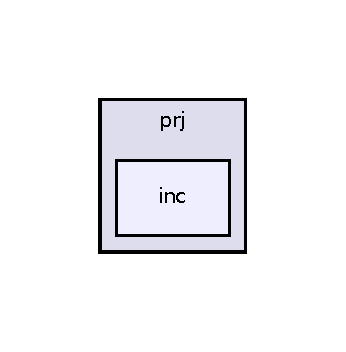
\includegraphics[width=166pt]{dir_da40416fce0315f7465b5a29481a9543_dep}
\end{center}
\end{figure}


\subsection*{Pliki}
\begin{DoxyCompactItemize}
\item 
plik \hyperlink{_l_zespolona_8hh}{LZespolona.hh}


\begin{DoxyCompactList}\small\item\em Klasa \hyperlink{class_l_zespolona}{LZespolona} sluzy do przechowywania liczby zespolonej w programie oraz do wykonywania operacji matematycznych na niej. \item\end{DoxyCompactList}

\item 
plik \hyperlink{_macierz_8hh}{Macierz.hh}


\begin{DoxyCompactList}\small\item\em Szablon Klasy \hyperlink{class_macierz}{Macierz} modeluje w programie macierz. \hyperlink{class_macierz}{Macierz} jest przechowywana w postaci Wektorow. Ich ilosc zalezy od rozmiaru Macierzy. Sklada sie z metody do obliczania wyznacznika i operatora indeksujacego,by bezposrednio odwolywac sie do macierzy. Sklada sie rowniez z funkcji arytmetycznych na macierzach. \item\end{DoxyCompactList}

\item 
plik \hyperlink{parametry_8hh}{parametry.hh}


\begin{DoxyCompactList}\small\item\em Struktura zawiera wszystkie pola odpowiadajace parametrom z jakimi moze zostac wywolany program. Posiada funkcje analizujaca parametry i Konwertujaca napis na liczbe. \item\end{DoxyCompactList}

\item 
plik \hyperlink{_uklad_rownan_liniowych_8hh}{UkladRownanLiniowych.hh}


\begin{DoxyCompactList}\small\item\em Klasa \hyperlink{class_uklad_rownan_liniowych}{UkladRownanLiniowych} modeluje w programie \hyperlink{class_macierz}{Macierz} wspolczynnikow rownania, wektor wyrazow wolnych. Sklada sie z metody do rozwiazania ukladu i wyswietlenia tego rozwiazania. \item\end{DoxyCompactList}

\item 
plik \hyperlink{_wektor_8hh}{Wektor.hh}


\begin{DoxyCompactList}\small\item\em Szablon Klasy wektor modeluje wektor w programie, przechowuje go jako 3elementowa tablice typu double Jej metody to operacje arytmetyczne na wektorach. \item\end{DoxyCompactList}

\end{DoxyCompactItemize}

\hypertarget{dir_5acca7a69a50425ed15b726665a92491}{
\section{Dokumentacja katalogu /home/fchodoro/kpo/zad/z7/Szablony/prj/}
\label{dir_5acca7a69a50425ed15b726665a92491}\index{Dokumentacja katalogu /home/fchodoro/kpo/zad/z7/Szablony/prj/@{Dokumentacja katalogu /home/fchodoro/kpo/zad/z7/Szablony/prj/}}
}


Directory dependency graph for /home/fchodoro/kpo/zad/z7/Szablony/prj/:\nopagebreak
\begin{figure}[H]
\begin{center}
\leavevmode
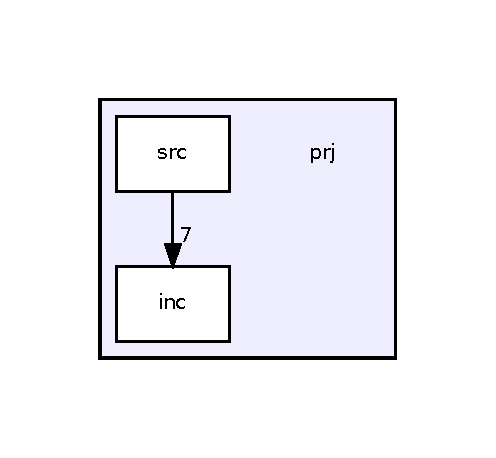
\includegraphics[width=238pt]{dir_5acca7a69a50425ed15b726665a92491_dep}
\end{center}
\end{figure}


\subsection*{Katalogi}
\begin{DoxyCompactItemize}
\item 
katalog \hyperlink{dir_da40416fce0315f7465b5a29481a9543}{inc}
\item 
katalog \hyperlink{dir_ea2c729999eb9d91c9fc78d011a1a046}{src}
\end{DoxyCompactItemize}

\hypertarget{dir_ea2c729999eb9d91c9fc78d011a1a046}{
\section{Dokumentacja katalogu /home/fchodoro/kpo/zad/z7/Szablony/prj/src/}
\label{dir_ea2c729999eb9d91c9fc78d011a1a046}\index{Dokumentacja katalogu /home/fchodoro/kpo/zad/z7/Szablony/prj/src/@{Dokumentacja katalogu /home/fchodoro/kpo/zad/z7/Szablony/prj/src/}}
}


Directory dependency graph for /home/fchodoro/kpo/zad/z7/Szablony/prj/src/:\nopagebreak
\begin{figure}[H]
\begin{center}
\leavevmode
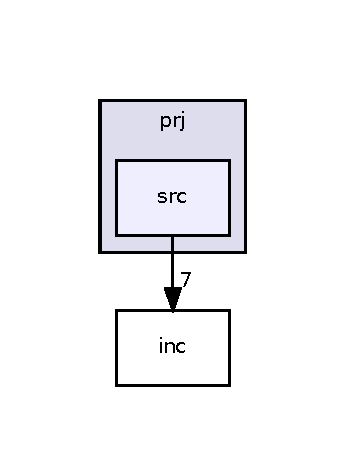
\includegraphics[width=166pt]{dir_ea2c729999eb9d91c9fc78d011a1a046_dep}
\end{center}
\end{figure}


\subsection*{Pliki}
\begin{DoxyCompactItemize}
\item 
plik \hyperlink{_l_zespolona_8cpp}{LZespolona.cpp}


\begin{DoxyCompactList}\small\item\em Definicja metod klasy LZesp. \item\end{DoxyCompactList}

\item 
plik \hyperlink{main_8cpp}{main.cpp}
\item 
plik \hyperlink{parametry_8cpp}{parametry.cpp}


\begin{DoxyCompactList}\small\item\em funkcje sluzacy do przetwarzania argumentow podanych w konsoli \item\end{DoxyCompactList}

\end{DoxyCompactItemize}

\chapter{Dokumentacja klas}
\hypertarget{class_l_zespolona}{
\section{Dokumentacja klasy LZespolona}
\label{class_l_zespolona}\index{LZespolona@{LZespolona}}
}


{\ttfamily \#include $<$LZespolona.hh$>$}

\subsection*{Metody publiczne}
\begin{DoxyCompactItemize}
\item 
\hyperlink{class_l_zespolona_a21fe2844a13cde80d7b00b891676296a}{LZespolona} ()
\item 
\hyperlink{class_l_zespolona_a46e0b6cdeb67e49640da865c0d01b671}{LZespolona} (double Re, double Im)
\item 
double \hyperlink{class_l_zespolona_a06ce2b4a22c1ca3f8d97e41b602f078e}{Re} () const 
\item 
double \hyperlink{class_l_zespolona_ad4057ab72b1471f38df277781baa0752}{Im} () const 
\item 
double \hyperlink{class_l_zespolona_a20dc93a471c88944e5c6efbc69b05f46}{operator\mbox{[}$\,$\mbox{]}} (int Ind) const 
\item 
double \& \hyperlink{class_l_zespolona_a77261afaa75950cb785bbffdff4b3cf7}{operator\mbox{[}$\,$\mbox{]}} (int Ind)
\item 
double \hyperlink{class_l_zespolona_aa9f4cab72cd025614fc5e2facb515e6e}{Modul} () const 
\begin{DoxyCompactList}\small\item\em Funkcja zwraca modul liczby zespolonej. \item\end{DoxyCompactList}\item 
int \hyperlink{class_l_zespolona_a4499e73b6e5b883df008be2694698f46}{operator==} (\hyperlink{class_l_zespolona}{LZespolona} const \&W)
\begin{DoxyCompactList}\small\item\em Funkcja operatorowa porownuje czesci rzeczywiste oraz czesci urojone liczby zespolonej. \item\end{DoxyCompactList}\item 
\hyperlink{class_l_zespolona}{LZespolona} \hyperlink{class_l_zespolona_aa744e58a7aede6f7318d4f9d3d9b650d}{operator+} (const \hyperlink{class_l_zespolona}{LZespolona} \&Q) const 
\begin{DoxyCompactList}\small\item\em Funkcja operatorowa dodaje liczby zespolone. \item\end{DoxyCompactList}\item 
\hyperlink{class_l_zespolona}{LZespolona} \hyperlink{class_l_zespolona_ad3875fdfa4e365029281d3dd0588dd68}{operator-\/} (const \hyperlink{class_l_zespolona}{LZespolona} \&B) const 
\begin{DoxyCompactList}\small\item\em Funkcja operatorowa odejmuje liczby zespolone. \item\end{DoxyCompactList}\item 
\hyperlink{class_l_zespolona}{LZespolona} \hyperlink{class_l_zespolona_a778727af986d4b8cddcbd089c6083644}{operator$\ast$} (const \hyperlink{class_l_zespolona}{LZespolona} \&Q) const 
\begin{DoxyCompactList}\small\item\em Funkcja operatorowa mnozy liczby zespolone. \item\end{DoxyCompactList}\item 
\hyperlink{class_l_zespolona}{LZespolona} \hyperlink{class_l_zespolona_aea67f672eb082a069c394f2aa832c65e}{operator/} (const \hyperlink{class_l_zespolona}{LZespolona} \&Q) const 
\begin{DoxyCompactList}\small\item\em Funkcja operatorowa sluzy do dzielenia liczby zespolonej przez zespolona. \item\end{DoxyCompactList}\item 
\hyperlink{class_l_zespolona}{LZespolona} \hyperlink{class_l_zespolona_a35b451d6d3bd0b0782bb1a73517e7f04}{operator-\/} () const 
\begin{DoxyCompactList}\small\item\em Funkcja operatorowa liczbe zespolona na przeciwna. \item\end{DoxyCompactList}\item 
const double \& \hyperlink{class_l_zespolona_aad1062d600b75272470a7b6e0b627000}{operator=} (const double \&a)
\begin{DoxyCompactList}\small\item\em Funkcja operatorowa = pozwala przypisac liczbe rzeczywista liczbie zespolonej. \item\end{DoxyCompactList}\item 
const int \& \hyperlink{class_l_zespolona_a1956d27ba5a7c68dd4e8adba81db23da}{operator=} (const int \&a)
\begin{DoxyCompactList}\small\item\em Funkcja operatorowa = pozwala przypisac liczbe calkowita liczbie zespolonej. \item\end{DoxyCompactList}\end{DoxyCompactItemize}
\subsection*{Atrybuty prywatne}
\begin{DoxyCompactItemize}
\item 
double \hyperlink{class_l_zespolona_a2c047555071a543fbe6a25e7ccb949c8}{\_\-re}
\item 
double \hyperlink{class_l_zespolona_af9a4d283c2939ea8b427e1eb0358cb2c}{\_\-im}
\end{DoxyCompactItemize}
\subsection*{Przyjaciele}
\begin{DoxyCompactItemize}
\item 
\hyperlink{class_l_zespolona}{LZespolona} \hyperlink{class_l_zespolona_a48f8e9c2b37ad5b3b8b964c25346b930}{operator+} (const double Liczba, const \hyperlink{class_l_zespolona}{LZespolona} \&Z)
\begin{DoxyCompactList}\small\item\em Funkcja operatorowa dodaje liczbe rzeczywista do liczby zespolonej. \item\end{DoxyCompactList}\item 
\hyperlink{class_l_zespolona}{LZespolona} \hyperlink{class_l_zespolona_aef47f3e429efa18ade4555f77df27014}{operator+} (const \hyperlink{class_l_zespolona}{LZespolona} \&Z, const double Liczba)
\begin{DoxyCompactList}\small\item\em Funkcja operatorowa dodaje liczbe rzeczywista do liczby zespolonej. \item\end{DoxyCompactList}\item 
\hyperlink{class_l_zespolona}{LZespolona} \hyperlink{class_l_zespolona_a896efd2b35c96235e487819ad646aebb}{operator$\ast$} (const double Liczba, const \hyperlink{class_l_zespolona}{LZespolona} \&Z)
\begin{DoxyCompactList}\small\item\em Funkcja operatorowa mnozy liczbe rzeczywista do liczby zespolonej. \item\end{DoxyCompactList}\item 
\hyperlink{class_l_zespolona}{LZespolona} \hyperlink{class_l_zespolona_a7cc8baeda5b16a42f0a193d3fbaf0a64}{operator$\ast$} (const \hyperlink{class_l_zespolona}{LZespolona} \&Z, const double Liczba)
\begin{DoxyCompactList}\small\item\em Funkcja operatorowa mnozy liczbe rzeczywista do liczby zespolonej. \item\end{DoxyCompactList}\item 
\hyperlink{class_l_zespolona}{LZespolona} \hyperlink{class_l_zespolona_afd6ac9993dc5c5279a990b98d607b2d4}{operator-\/} (const \hyperlink{class_l_zespolona}{LZespolona} \&Z, const double Liczba)
\begin{DoxyCompactList}\small\item\em Funkcja operatorowa odejmuje liczbe rzeczywista od liczby zespolonej. \item\end{DoxyCompactList}\item 
\hyperlink{class_l_zespolona}{LZespolona} \hyperlink{class_l_zespolona_adde8e8baef5452a13cc50c8c72e8d397}{operator/} (const \hyperlink{class_l_zespolona}{LZespolona} \&Z, const double Liczba)
\begin{DoxyCompactList}\small\item\em Funkcja operatorowa dzieli liczbe zespolona przez liczbe zespolona. \item\end{DoxyCompactList}\end{DoxyCompactItemize}


\subsection{Opis szczegółowy}


Definicja w linii 10 pliku LZespolona.hh.



\subsection{Dokumentacja konstruktora i destruktora}
\hypertarget{class_l_zespolona_a21fe2844a13cde80d7b00b891676296a}{
\index{LZespolona@{LZespolona}!LZespolona@{LZespolona}}
\index{LZespolona@{LZespolona}!LZespolona@{LZespolona}}
\subsubsection[{LZespolona}]{\setlength{\rightskip}{0pt plus 5cm}LZespolona::LZespolona (
\begin{DoxyParamCaption}
{}
\end{DoxyParamCaption}
)\hspace{0.3cm}{\ttfamily  \mbox{[}inline\mbox{]}}}}
\label{class_l_zespolona_a21fe2844a13cde80d7b00b891676296a}
brief Domniemany konstruktor liczby zespolonej 

Definicja w linii 26 pliku LZespolona.hh.

\hypertarget{class_l_zespolona_a46e0b6cdeb67e49640da865c0d01b671}{
\index{LZespolona@{LZespolona}!LZespolona@{LZespolona}}
\index{LZespolona@{LZespolona}!LZespolona@{LZespolona}}
\subsubsection[{LZespolona}]{\setlength{\rightskip}{0pt plus 5cm}LZespolona::LZespolona (
\begin{DoxyParamCaption}
\item[{double}]{ Re, }
\item[{double}]{ Im}
\end{DoxyParamCaption}
)\hspace{0.3cm}{\ttfamily  \mbox{[}inline\mbox{]}}}}
\label{class_l_zespolona_a46e0b6cdeb67e49640da865c0d01b671}
brief Konstruktor liczby zespolonej z 2 argumentami typu double 

Definicja w linii 30 pliku LZespolona.hh.



\subsection{Dokumentacja funkcji składowych}
\hypertarget{class_l_zespolona_ad4057ab72b1471f38df277781baa0752}{
\index{LZespolona@{LZespolona}!Im@{Im}}
\index{Im@{Im}!LZespolona@{LZespolona}}
\subsubsection[{Im}]{\setlength{\rightskip}{0pt plus 5cm}double LZespolona::Im (
\begin{DoxyParamCaption}
{}
\end{DoxyParamCaption}
) const\hspace{0.3cm}{\ttfamily  \mbox{[}inline\mbox{]}}}}
\label{class_l_zespolona_ad4057ab72b1471f38df277781baa0752}
brief Funkcja zwraca czesc urojona liczby zespolonej 

Definicja w linii 39 pliku LZespolona.hh.

\hypertarget{class_l_zespolona_aa9f4cab72cd025614fc5e2facb515e6e}{
\index{LZespolona@{LZespolona}!Modul@{Modul}}
\index{Modul@{Modul}!LZespolona@{LZespolona}}
\subsubsection[{Modul}]{\setlength{\rightskip}{0pt plus 5cm}double LZespolona::Modul (
\begin{DoxyParamCaption}
{}
\end{DoxyParamCaption}
) const}}
\label{class_l_zespolona_aa9f4cab72cd025614fc5e2facb515e6e}
brief Funkcja zwraca modul liczby zespolonej

\begin{DoxyReturn}{Zwraca}
zwraca modul liczby zespolonej 
\end{DoxyReturn}
\begin{DoxyPrecond}{Warunek wstępny}
Poprawne wczytanie liczby zespolonej 
\end{DoxyPrecond}


Definicja w linii 18 pliku LZespolona.cpp.



Oto graf wywołań dla tej funkcji:\nopagebreak
\begin{figure}[H]
\begin{center}
\leavevmode
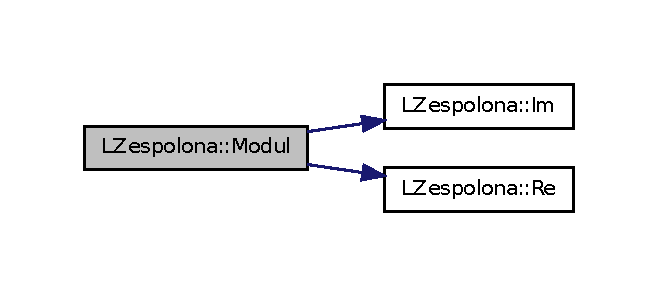
\includegraphics[width=316pt]{class_l_zespolona_aa9f4cab72cd025614fc5e2facb515e6e_cgraph}
\end{center}
\end{figure}


\hypertarget{class_l_zespolona_a778727af986d4b8cddcbd089c6083644}{
\index{LZespolona@{LZespolona}!operator$\ast$@{operator$\ast$}}
\index{operator$\ast$@{operator$\ast$}!LZespolona@{LZespolona}}
\subsubsection[{operator$\ast$}]{\setlength{\rightskip}{0pt plus 5cm}{\bf LZespolona} LZespolona::operator$\ast$ (
\begin{DoxyParamCaption}
\item[{const {\bf LZespolona} \&}]{ Q}
\end{DoxyParamCaption}
) const}}
\label{class_l_zespolona_a778727af986d4b8cddcbd089c6083644}
brief Mnozenie liczb zespolonych


\begin{DoxyParams}{Parametry}
\item[\mbox{\tt[in]} {\em Q}]-\/ liczba zespolona. \end{DoxyParams}
\begin{DoxyReturn}{Zwraca}
Zwraca liczbe zespolona. 
\end{DoxyReturn}
\begin{DoxyPrecond}{Warunek wstępny}
Poprawne wczytanie dwoch liczb zespolonych 
\end{DoxyPrecond}


Definicja w linii 70 pliku LZespolona.cpp.

\hypertarget{class_l_zespolona_aa744e58a7aede6f7318d4f9d3d9b650d}{
\index{LZespolona@{LZespolona}!operator+@{operator+}}
\index{operator+@{operator+}!LZespolona@{LZespolona}}
\subsubsection[{operator+}]{\setlength{\rightskip}{0pt plus 5cm}{\bf LZespolona} LZespolona::operator+ (
\begin{DoxyParamCaption}
\item[{const {\bf LZespolona} \&}]{ Q}
\end{DoxyParamCaption}
) const}}
\label{class_l_zespolona_aa744e58a7aede6f7318d4f9d3d9b650d}
brief Dodawanie liczb zespolonych


\begin{DoxyParams}{Parametry}
\item[\mbox{\tt[in]} {\em Q}]-\/ liczba zespolona. \end{DoxyParams}
\begin{DoxyReturn}{Zwraca}
Zwraca liczbe zespolona. 
\end{DoxyReturn}
\begin{DoxyPrecond}{Warunek wstępny}
Poprawne wczytanie dwoch liczb zespolonych 
\end{DoxyPrecond}


Definicja w linii 29 pliku LZespolona.cpp.

\hypertarget{class_l_zespolona_ad3875fdfa4e365029281d3dd0588dd68}{
\index{LZespolona@{LZespolona}!operator-\/@{operator-\/}}
\index{operator-\/@{operator-\/}!LZespolona@{LZespolona}}
\subsubsection[{operator-\/}]{\setlength{\rightskip}{0pt plus 5cm}{\bf LZespolona} LZespolona::operator-\/ (
\begin{DoxyParamCaption}
\item[{const {\bf LZespolona} \&}]{ B}
\end{DoxyParamCaption}
) const}}
\label{class_l_zespolona_ad3875fdfa4e365029281d3dd0588dd68}
brief Odejmowanie liczb zespolonych


\begin{DoxyParams}{Parametry}
\item[\mbox{\tt[in]} {\em B}]-\/ liczba zespolona. \end{DoxyParams}
\begin{DoxyReturn}{Zwraca}
Zwraca liczbe zespolona. 
\end{DoxyReturn}
\begin{DoxyPrecond}{Warunek wstępny}
Poprawne wczytanie dwoch liczb zespolonych 
\end{DoxyPrecond}


Definicja w linii 56 pliku LZespolona.cpp.

\hypertarget{class_l_zespolona_a35b451d6d3bd0b0782bb1a73517e7f04}{
\index{LZespolona@{LZespolona}!operator-\/@{operator-\/}}
\index{operator-\/@{operator-\/}!LZespolona@{LZespolona}}
\subsubsection[{operator-\/}]{\setlength{\rightskip}{0pt plus 5cm}{\bf LZespolona} LZespolona::operator-\/ (
\begin{DoxyParamCaption}
{}
\end{DoxyParamCaption}
) const}}
\label{class_l_zespolona_a35b451d6d3bd0b0782bb1a73517e7f04}
brief Odejmowanie liczb zespolonych

\begin{DoxyReturn}{Zwraca}
Zwraca liczbe zespolona. 
\end{DoxyReturn}
\begin{DoxyPrecond}{Warunek wstępny}
Poprawne wczytanie liczby zespolonej 
\end{DoxyPrecond}


Definicja w linii 42 pliku LZespolona.cpp.

\hypertarget{class_l_zespolona_aea67f672eb082a069c394f2aa832c65e}{
\index{LZespolona@{LZespolona}!operator/@{operator/}}
\index{operator/@{operator/}!LZespolona@{LZespolona}}
\subsubsection[{operator/}]{\setlength{\rightskip}{0pt plus 5cm}{\bf LZespolona} LZespolona::operator/ (
\begin{DoxyParamCaption}
\item[{const {\bf LZespolona} \&}]{ Q}
\end{DoxyParamCaption}
) const}}
\label{class_l_zespolona_aea67f672eb082a069c394f2aa832c65e}
brief Dzielenie liczb zespolonych


\begin{DoxyParams}{Parametry}
\item[\mbox{\tt[in]} {\em Q}]-\/ liczba zespolona. \end{DoxyParams}
\begin{DoxyReturn}{Zwraca}
Zwraca liczbe zespolona. 
\end{DoxyReturn}
\begin{DoxyPrecond}{Warunek wstępny}
Poprawne wczytanie dwoch liczb zespolonych 
\end{DoxyPrecond}


Definicja w linii 85 pliku LZespolona.cpp.

\hypertarget{class_l_zespolona_a1956d27ba5a7c68dd4e8adba81db23da}{
\index{LZespolona@{LZespolona}!operator=@{operator=}}
\index{operator=@{operator=}!LZespolona@{LZespolona}}
\subsubsection[{operator=}]{\setlength{\rightskip}{0pt plus 5cm}const int \& LZespolona::operator= (
\begin{DoxyParamCaption}
\item[{const int \&}]{ a}
\end{DoxyParamCaption}
)}}
\label{class_l_zespolona_a1956d27ba5a7c68dd4e8adba81db23da}
brief Przypisanie wartosci calkowitej liczbie zespolonej


\begin{DoxyParams}{Parametry}
\item[\mbox{\tt[in]} {\em \&a}]-\/ referencja do liczby calkowitej \end{DoxyParams}
\begin{DoxyReturn}{Zwraca}
Zwraca referencje do liczby calkowitej 
\end{DoxyReturn}
\begin{DoxyPostcond}{Warunek końcowy}
Liczba zostaje zrzutowana na typ rzeczywisty 
\end{DoxyPostcond}


Definicja w linii 230 pliku LZespolona.cpp.

\hypertarget{class_l_zespolona_aad1062d600b75272470a7b6e0b627000}{
\index{LZespolona@{LZespolona}!operator=@{operator=}}
\index{operator=@{operator=}!LZespolona@{LZespolona}}
\subsubsection[{operator=}]{\setlength{\rightskip}{0pt plus 5cm}const double \& LZespolona::operator= (
\begin{DoxyParamCaption}
\item[{const double \&}]{ a}
\end{DoxyParamCaption}
)}}
\label{class_l_zespolona_aad1062d600b75272470a7b6e0b627000}
brief Przypisanie wartosci rzeczywistej liczbie zespolonej


\begin{DoxyParams}{Parametry}
\item[\mbox{\tt[in]} {\em \&a}]-\/ referencja do liczby rzeczywistej \end{DoxyParams}
\begin{DoxyReturn}{Zwraca}
Zwraca referencje do liczby rzeczywistej 
\end{DoxyReturn}


Definicja w linii 216 pliku LZespolona.cpp.

\hypertarget{class_l_zespolona_a4499e73b6e5b883df008be2694698f46}{
\index{LZespolona@{LZespolona}!operator==@{operator==}}
\index{operator==@{operator==}!LZespolona@{LZespolona}}
\subsubsection[{operator==}]{\setlength{\rightskip}{0pt plus 5cm}int LZespolona::operator== (
\begin{DoxyParamCaption}
\item[{{\bf LZespolona} const \&}]{ W}
\end{DoxyParamCaption}
)}}
\label{class_l_zespolona_a4499e73b6e5b883df008be2694698f46}
brief Przeciazenie operatora porownania dla liczb zespolonych


\begin{DoxyParams}{Parametry}
\item[\mbox{\tt[in]} {\em W}]-\/ liczba zespolona. \end{DoxyParams}
\begin{DoxyReturn}{Zwraca}
Zwraca liczbe zespolona. 
\end{DoxyReturn}
\begin{DoxyPrecond}{Warunek wstępny}
Poprawne wczytanie dwoch liczb zespolonych 
\end{DoxyPrecond}


Definicja w linii 100 pliku LZespolona.cpp.

\hypertarget{class_l_zespolona_a20dc93a471c88944e5c6efbc69b05f46}{
\index{LZespolona@{LZespolona}!operator\mbox{[}\mbox{]}@{operator[]}}
\index{operator\mbox{[}\mbox{]}@{operator[]}!LZespolona@{LZespolona}}
\subsubsection[{operator[]}]{\setlength{\rightskip}{0pt plus 5cm}double LZespolona::operator\mbox{[}$\,$\mbox{]} (
\begin{DoxyParamCaption}
\item[{int}]{ Ind}
\end{DoxyParamCaption}
) const\hspace{0.3cm}{\ttfamily  \mbox{[}inline\mbox{]}}}}
\label{class_l_zespolona_a20dc93a471c88944e5c6efbc69b05f46}
brief Przeciazenie operatora indeksowania dla liczby zespolonej 

Definicja w linii 43 pliku LZespolona.hh.

\hypertarget{class_l_zespolona_a77261afaa75950cb785bbffdff4b3cf7}{
\index{LZespolona@{LZespolona}!operator\mbox{[}\mbox{]}@{operator[]}}
\index{operator\mbox{[}\mbox{]}@{operator[]}!LZespolona@{LZespolona}}
\subsubsection[{operator[]}]{\setlength{\rightskip}{0pt plus 5cm}double\& LZespolona::operator\mbox{[}$\,$\mbox{]} (
\begin{DoxyParamCaption}
\item[{int}]{ Ind}
\end{DoxyParamCaption}
)\hspace{0.3cm}{\ttfamily  \mbox{[}inline\mbox{]}}}}
\label{class_l_zespolona_a77261afaa75950cb785bbffdff4b3cf7}
brief Przeciazenie operatora indeksowania dla liczby zespolonej 

Definicja w linii 47 pliku LZespolona.hh.

\hypertarget{class_l_zespolona_a06ce2b4a22c1ca3f8d97e41b602f078e}{
\index{LZespolona@{LZespolona}!Re@{Re}}
\index{Re@{Re}!LZespolona@{LZespolona}}
\subsubsection[{Re}]{\setlength{\rightskip}{0pt plus 5cm}double LZespolona::Re (
\begin{DoxyParamCaption}
{}
\end{DoxyParamCaption}
) const\hspace{0.3cm}{\ttfamily  \mbox{[}inline\mbox{]}}}}
\label{class_l_zespolona_a06ce2b4a22c1ca3f8d97e41b602f078e}
brief Funkcja zwraca czesc rzeczywista liczby zespolonej 

Definicja w linii 35 pliku LZespolona.hh.



\subsection{Dokumentacja przyjaciół i funkcji związanych}
\hypertarget{class_l_zespolona_a896efd2b35c96235e487819ad646aebb}{
\index{LZespolona@{LZespolona}!operator$\ast$@{operator$\ast$}}
\index{operator$\ast$@{operator$\ast$}!LZespolona@{LZespolona}}
\subsubsection[{operator$\ast$}]{\setlength{\rightskip}{0pt plus 5cm}{\bf LZespolona} operator$\ast$ (
\begin{DoxyParamCaption}
\item[{const double}]{ Liczba, }
\item[{const {\bf LZespolona} \&}]{ Z}
\end{DoxyParamCaption}
)\hspace{0.3cm}{\ttfamily  \mbox{[}friend\mbox{]}}}}
\label{class_l_zespolona_a896efd2b35c96235e487819ad646aebb}
briefMnozenie liczby(niezespolonej) z liczba niezespolona


\begin{DoxyParams}{Parametry}
\item[{\em Z}]-\/ liczba zespolona. \item[{\em Liczba}]-\/ liczba rzeczywista \end{DoxyParams}
\begin{DoxyReturn}{Zwraca}
Zwraca liczbe zespolona. 
\end{DoxyReturn}
\begin{DoxyPrecond}{Warunek wstępny}
Poprawne wczytanie dwoch liczb zespolonych 
\end{DoxyPrecond}


Definicja w linii 158 pliku LZespolona.cpp.

\hypertarget{class_l_zespolona_a7cc8baeda5b16a42f0a193d3fbaf0a64}{
\index{LZespolona@{LZespolona}!operator$\ast$@{operator$\ast$}}
\index{operator$\ast$@{operator$\ast$}!LZespolona@{LZespolona}}
\subsubsection[{operator$\ast$}]{\setlength{\rightskip}{0pt plus 5cm}{\bf LZespolona} operator$\ast$ (
\begin{DoxyParamCaption}
\item[{const {\bf LZespolona} \&}]{ Z, }
\item[{const double}]{ Liczba}
\end{DoxyParamCaption}
)\hspace{0.3cm}{\ttfamily  \mbox{[}friend\mbox{]}}}}
\label{class_l_zespolona_a7cc8baeda5b16a42f0a193d3fbaf0a64}
brief Mnozenie liczby(niezespolonej) z liczba niezespolona


\begin{DoxyParams}{Parametry}
\item[{\em Z}]-\/ liczba zespolona. \item[{\em Liczba}]-\/ liczba rzeczywista \end{DoxyParams}
\begin{DoxyReturn}{Zwraca}
Zwraca liczbe zespolona. 
\end{DoxyReturn}
\begin{DoxyPrecond}{Warunek wstępny}
Poprawne wczytanie dwoch liczb zespolonych 
\end{DoxyPrecond}


Definicja w linii 174 pliku LZespolona.cpp.

\hypertarget{class_l_zespolona_aef47f3e429efa18ade4555f77df27014}{
\index{LZespolona@{LZespolona}!operator+@{operator+}}
\index{operator+@{operator+}!LZespolona@{LZespolona}}
\subsubsection[{operator+}]{\setlength{\rightskip}{0pt plus 5cm}{\bf LZespolona} operator+ (
\begin{DoxyParamCaption}
\item[{const {\bf LZespolona} \&}]{ Z, }
\item[{const double}]{ Liczba}
\end{DoxyParamCaption}
)\hspace{0.3cm}{\ttfamily  \mbox{[}friend\mbox{]}}}}
\label{class_l_zespolona_aef47f3e429efa18ade4555f77df27014}
brief Dodawanie liczby(nie zespolonej) do liczby zespolonej


\begin{DoxyParams}{Parametry}
\item[{\em Z}]-\/ liczba zespolona. \item[{\em Liczba}]-\/ liczba rzeczywista \end{DoxyParams}
\begin{DoxyReturn}{Zwraca}
Zwraca liczbe zespolona. 
\end{DoxyReturn}
\begin{DoxyPrecond}{Warunek wstępny}
Poprawne wczytanie dwoch liczb zespolonych 
\end{DoxyPrecond}


Definicja w linii 128 pliku LZespolona.cpp.

\hypertarget{class_l_zespolona_a48f8e9c2b37ad5b3b8b964c25346b930}{
\index{LZespolona@{LZespolona}!operator+@{operator+}}
\index{operator+@{operator+}!LZespolona@{LZespolona}}
\subsubsection[{operator+}]{\setlength{\rightskip}{0pt plus 5cm}{\bf LZespolona} operator+ (
\begin{DoxyParamCaption}
\item[{const double}]{ Liczba, }
\item[{const {\bf LZespolona} \&}]{ Z}
\end{DoxyParamCaption}
)\hspace{0.3cm}{\ttfamily  \mbox{[}friend\mbox{]}}}}
\label{class_l_zespolona_a48f8e9c2b37ad5b3b8b964c25346b930}
brief Dodawanie liczby(nie zespolonej) do liczby zespolonej


\begin{DoxyParams}{Parametry}
\item[{\em Z}]-\/ liczba zespolona. \item[{\em Liczba}]-\/ liczba rzeczywista \end{DoxyParams}
\begin{DoxyReturn}{Zwraca}
Zwraca liczbe zespolona. 
\end{DoxyReturn}
\begin{DoxyPrecond}{Warunek wstępny}
Poprawne wczytanie dwoch liczb zespolonych 
\end{DoxyPrecond}


Definicja w linii 113 pliku LZespolona.cpp.

\hypertarget{class_l_zespolona_afd6ac9993dc5c5279a990b98d607b2d4}{
\index{LZespolona@{LZespolona}!operator-\/@{operator-\/}}
\index{operator-\/@{operator-\/}!LZespolona@{LZespolona}}
\subsubsection[{operator-\/}]{\setlength{\rightskip}{0pt plus 5cm}{\bf LZespolona} operator-\/ (
\begin{DoxyParamCaption}
\item[{const {\bf LZespolona} \&}]{ Z, }
\item[{const double}]{ Liczba}
\end{DoxyParamCaption}
)\hspace{0.3cm}{\ttfamily  \mbox{[}friend\mbox{]}}}}
\label{class_l_zespolona_afd6ac9993dc5c5279a990b98d607b2d4}
brief Odejmowanie od liczby zespolonej liczby niezespolonej


\begin{DoxyParams}{Parametry}
\item[{\em Z}]-\/ liczba zespolona. \item[{\em Liczba}]-\/ liczba rzeczywista \end{DoxyParams}
\begin{DoxyReturn}{Zwraca}
Zwraca liczbe zespolona. 
\end{DoxyReturn}
\begin{DoxyPrecond}{Warunek wstępny}
Poprawne wczytanie dwoch liczb zespolonych 
\end{DoxyPrecond}


Definicja w linii 143 pliku LZespolona.cpp.

\hypertarget{class_l_zespolona_adde8e8baef5452a13cc50c8c72e8d397}{
\index{LZespolona@{LZespolona}!operator/@{operator/}}
\index{operator/@{operator/}!LZespolona@{LZespolona}}
\subsubsection[{operator/}]{\setlength{\rightskip}{0pt plus 5cm}{\bf LZespolona} operator/ (
\begin{DoxyParamCaption}
\item[{const {\bf LZespolona} \&}]{ Z, }
\item[{const double}]{ Liczba}
\end{DoxyParamCaption}
)\hspace{0.3cm}{\ttfamily  \mbox{[}friend\mbox{]}}}}
\label{class_l_zespolona_adde8e8baef5452a13cc50c8c72e8d397}
brief Dzielenie liczby zespolonej przez liczbe niezespolona


\begin{DoxyParams}{Parametry}
\item[{\em Z}]-\/ liczba zespolona. \item[{\em Liczba}]-\/ liczba rzeczywista \end{DoxyParams}
\begin{DoxyReturn}{Zwraca}
Zwraca liczbe zespolona. 
\end{DoxyReturn}
\begin{DoxyPrecond}{Warunek wstępny}
Poprawne wczytanie dwoch liczb zespolonych 
\end{DoxyPrecond}


Definicja w linii 190 pliku LZespolona.cpp.



\subsection{Dokumentacja atrybutów składowych}
\hypertarget{class_l_zespolona_af9a4d283c2939ea8b427e1eb0358cb2c}{
\index{LZespolona@{LZespolona}!\_\-im@{\_\-im}}
\index{\_\-im@{\_\-im}!LZespolona@{LZespolona}}
\subsubsection[{\_\-im}]{\setlength{\rightskip}{0pt plus 5cm}double {\bf LZespolona::\_\-im}\hspace{0.3cm}{\ttfamily  \mbox{[}private\mbox{]}}}}
\label{class_l_zespolona_af9a4d283c2939ea8b427e1eb0358cb2c}
brief czesc urojona liczby zespolonej 

Definicja w linii 19 pliku LZespolona.hh.

\hypertarget{class_l_zespolona_a2c047555071a543fbe6a25e7ccb949c8}{
\index{LZespolona@{LZespolona}!\_\-re@{\_\-re}}
\index{\_\-re@{\_\-re}!LZespolona@{LZespolona}}
\subsubsection[{\_\-re}]{\setlength{\rightskip}{0pt plus 5cm}double {\bf LZespolona::\_\-re}\hspace{0.3cm}{\ttfamily  \mbox{[}private\mbox{]}}}}
\label{class_l_zespolona_a2c047555071a543fbe6a25e7ccb949c8}
brief czesc rzeczywista liczby zespolonej 

Definicja w linii 15 pliku LZespolona.hh.



Dokumentacja dla tej klasy została wygenerowana z plików:\begin{DoxyCompactItemize}
\item 
\hyperlink{_l_zespolona_8hh}{LZespolona.hh}\item 
\hyperlink{_l_zespolona_8cpp}{LZespolona.cpp}\end{DoxyCompactItemize}

\hypertarget{class_macierz}{
\section{Dokumentacja szablonu klasy Macierz$<$ Typ, ROZMIAR $>$}
\label{class_macierz}\index{Macierz@{Macierz}}
}


{\ttfamily \#include $<$Macierz.hh$>$}

\subsection*{Metody publiczne}
\begin{DoxyCompactItemize}
\item 
\hyperlink{class_wektor}{Wektor}$<$ Typ, ROZMIAR $>$ \& \hyperlink{class_macierz_aaa9522b86fd7a63646fd07890e45dd11}{operator\mbox{[}$\,$\mbox{]}} (int Wie)
\begin{DoxyCompactList}\small\item\em Przeciazenia indeksow dla macierzy. Funkcja operatorowa \mbox{[}\mbox{]} sluzy do indeksowania klasy \hyperlink{class_macierz}{Macierz},by moc odnosic sie w bezposredni sposob do tablicy typu \hyperlink{class_wektor}{Wektor} tej klasy. \item\end{DoxyCompactList}\item 
const \hyperlink{class_wektor}{Wektor}$<$ Typ, ROZMIAR $>$ \& \hyperlink{class_macierz_abb153212ae62cdf841f96320f891cfb2}{operator\mbox{[}$\,$\mbox{]}} (int Wie) const 
\begin{DoxyCompactList}\small\item\em Przeciazenia indeksow dla macierzy. Funkcja operatorowa \mbox{[}\mbox{]} sluzy do indeksowania klasy \hyperlink{class_macierz}{Macierz},by moc odnosic sie w bezposredni sposob do tablicy typu \hyperlink{class_wektor}{Wektor} tej klasy. \item\end{DoxyCompactList}\item 
\hyperlink{class_macierz}{Macierz}$<$ Typ, ROZMIAR $>$ \hyperlink{class_macierz_ae8f58657a41da4c9c54c4f0ed85f554e}{operator$\ast$} (\hyperlink{class_macierz}{Macierz}$<$ Typ, ROZMIAR $>$ \&Mac2)
\begin{DoxyCompactList}\small\item\em Szablon funkcji operatorowej $\ast$ sluzy do mnozenia macierzy przez macierz. \item\end{DoxyCompactList}\item 
\hyperlink{class_wektor}{Wektor}$<$ Typ, ROZMIAR $>$ \hyperlink{class_macierz_ac60295eba85e578dc300b1c3f0431684}{operator$\ast$} (const \hyperlink{class_wektor}{Wektor}$<$ Typ, ROZMIAR $>$ Wek) const 
\begin{DoxyCompactList}\small\item\em Szablon funkcji operatorowej $\ast$ sluzy do mnozenia macierzy przez wektor. \item\end{DoxyCompactList}\item 
\hyperlink{class_wektor}{Wektor}$<$ Typ, ROZMIAR $>$ \& \hyperlink{class_macierz_ab94e869cad4bc457c5796e20d5c34348}{Transpozycja} ()
\begin{DoxyCompactList}\small\item\em Szablon funkcji Transpozycja sluzy do Transponowania macierzy, czyli. \item\end{DoxyCompactList}\item 
double \hyperlink{class_macierz_a3d8e9e4fee3850b78b0caf5215b34893}{SortowanieWierszy} ()
\begin{DoxyCompactList}\small\item\em Szablon funkcji SortowanieWierszy sluzy do zamiany wierszy w macierzy. \item\end{DoxyCompactList}\item 
Typ \hyperlink{class_macierz_a57a50f518945cd9152a88f367cb23e9e}{ObliczWyznacznik} () const 
\begin{DoxyCompactList}\small\item\em Szablon funkcji ObliczWyznacznik sluzy do obliczenia wyznacznika macierzy o zadanym rozmiarze. \item\end{DoxyCompactList}\end{DoxyCompactItemize}
\subsection*{Atrybuty prywatne}
\begin{DoxyCompactItemize}
\item 
\hyperlink{class_wektor}{Wektor}$<$ Typ, ROZMIAR $>$ \hyperlink{class_macierz_a2b7a2db3b700ad190ff592c470a8afb3}{\_\-Wiersz} \mbox{[}ROZMIAR\mbox{]}
\begin{DoxyCompactList}\small\item\em Szablon macierzy skladajacej sie z wektorow. \item\end{DoxyCompactList}\end{DoxyCompactItemize}


\subsection{Opis szczegółowy}
\subsubsection*{template$<$typename Typ, int ROZMIAR$>$ class Macierz$<$ Typ, ROZMIAR $>$}



Definicja w linii 18 pliku Macierz.hh.



\subsection{Dokumentacja funkcji składowych}
\hypertarget{class_macierz_a57a50f518945cd9152a88f367cb23e9e}{
\index{Macierz@{Macierz}!ObliczWyznacznik@{ObliczWyznacznik}}
\index{ObliczWyznacznik@{ObliczWyznacznik}!Macierz@{Macierz}}
\subsubsection[{ObliczWyznacznik}]{\setlength{\rightskip}{0pt plus 5cm}template$<$typename Typ , int ROZMIAR$>$ Typ {\bf Macierz}$<$ Typ, ROZMIAR $>$::ObliczWyznacznik (
\begin{DoxyParamCaption}
{}
\end{DoxyParamCaption}
) const}}
\label{class_macierz_a57a50f518945cd9152a88f367cb23e9e}
Szablon funkcji ObliczWyznacznik sluzy do obliczenia wyznacznika macierzy o zadanym rozmiarze. Zwraca element typu bool Jej elementem jest referencja do macierzy.

\begin{DoxyPrecond}{Warunek wstępny}
Poprawnie wczytana macierz 
\end{DoxyPrecond}
\begin{DoxyReturn}{Zwraca}
Zostaje obliczony wyznacznik 

wartosc true gdy wyznacznik rozny od 0, false,gdy rowny 0. 
\end{DoxyReturn}


Definicja w linii 203 pliku Macierz.hh.



Oto graf wywołań dla tej funkcji:\nopagebreak
\begin{figure}[H]
\begin{center}
\leavevmode
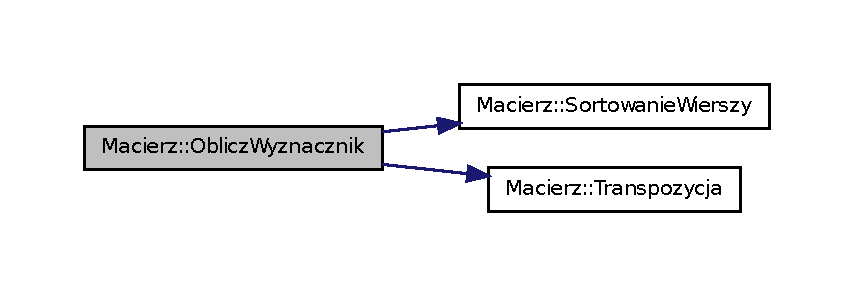
\includegraphics[width=400pt]{class_macierz_a57a50f518945cd9152a88f367cb23e9e_cgraph}
\end{center}
\end{figure}


\hypertarget{class_macierz_ac60295eba85e578dc300b1c3f0431684}{
\index{Macierz@{Macierz}!operator$\ast$@{operator$\ast$}}
\index{operator$\ast$@{operator$\ast$}!Macierz@{Macierz}}
\subsubsection[{operator$\ast$}]{\setlength{\rightskip}{0pt plus 5cm}template$<$typename Typ , int ROZMIAR$>$ {\bf Wektor}$<$ Typ, ROZMIAR $>$ {\bf Macierz}$<$ Typ, ROZMIAR $>$::operator$\ast$ (
\begin{DoxyParamCaption}
\item[{const {\bf Wektor}$<$ Typ, ROZMIAR $>$}]{ Wek}
\end{DoxyParamCaption}
) const}}
\label{class_macierz_ac60295eba85e578dc300b1c3f0431684}

\begin{DoxyParams}{Parametry}
\item[\mbox{\tt[in]} {\em Wek}]-\/ wektor \end{DoxyParams}
\begin{DoxyPrecond}{Warunek wstępny}
poprawne wczytanie wektora i macierzy 
\end{DoxyPrecond}
\begin{DoxyReturn}{Zwraca}
mnozenie macierzy przez wektor, wynik jako wartosc zwracana przez funkcje 
\end{DoxyReturn}


Definicja w linii 113 pliku Macierz.hh.

\hypertarget{class_macierz_ae8f58657a41da4c9c54c4f0ed85f554e}{
\index{Macierz@{Macierz}!operator$\ast$@{operator$\ast$}}
\index{operator$\ast$@{operator$\ast$}!Macierz@{Macierz}}
\subsubsection[{operator$\ast$}]{\setlength{\rightskip}{0pt plus 5cm}template$<$typename Typ , int ROZMIAR$>$ {\bf Macierz}$<$ Typ, ROZMIAR $>$ {\bf Macierz}$<$ Typ, ROZMIAR $>$::operator$\ast$ (
\begin{DoxyParamCaption}
\item[{{\bf Macierz}$<$ Typ, ROZMIAR $>$ \&}]{ Mac2}
\end{DoxyParamCaption}
)}}
\label{class_macierz_ae8f58657a41da4c9c54c4f0ed85f554e}
\begin{DoxyReturn}{Zwraca}
element typu \hyperlink{class_macierz}{Macierz} 
\end{DoxyReturn}

\begin{DoxyParams}{Parametry}
\item[\mbox{\tt[in]} {\em \&Mac2}]-\/ szablon referencji do klasy typu \hyperlink{class_macierz}{Macierz} \end{DoxyParams}
\begin{DoxyPrecond}{Warunek wstępny}
poprawne wczytanie macierzy 
\end{DoxyPrecond}
\begin{DoxyReturn}{Zwraca}
mnozenie macierzy przez macierz, wynik jako wartosc zwracana przez funkcje 
\end{DoxyReturn}


Definicja w linii 149 pliku Macierz.hh.



Oto graf wywołań dla tej funkcji:\nopagebreak
\begin{figure}[H]
\begin{center}
\leavevmode
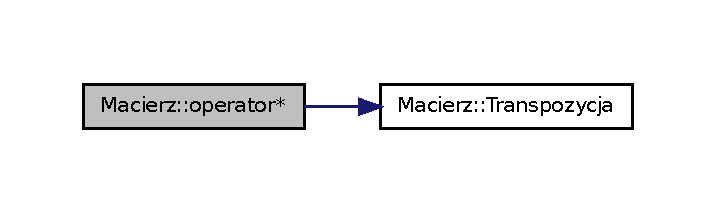
\includegraphics[width=344pt]{class_macierz_ae8f58657a41da4c9c54c4f0ed85f554e_cgraph}
\end{center}
\end{figure}


\hypertarget{class_macierz_aaa9522b86fd7a63646fd07890e45dd11}{
\index{Macierz@{Macierz}!operator\mbox{[}\mbox{]}@{operator[]}}
\index{operator\mbox{[}\mbox{]}@{operator[]}!Macierz@{Macierz}}
\subsubsection[{operator[]}]{\setlength{\rightskip}{0pt plus 5cm}template$<$typename Typ, int ROZMIAR$>$ {\bf Wektor}$<$Typ,ROZMIAR$>$\& {\bf Macierz}$<$ Typ, ROZMIAR $>$::operator\mbox{[}$\,$\mbox{]} (
\begin{DoxyParamCaption}
\item[{int}]{ Wie}
\end{DoxyParamCaption}
)\hspace{0.3cm}{\ttfamily  \mbox{[}inline\mbox{]}}}}
\label{class_macierz_aaa9522b86fd7a63646fd07890e45dd11}

\begin{DoxyParams}{Parametry}
\item[\mbox{\tt[in]} {\em Wie}]-\/ numer wiersza macierzy \end{DoxyParams}
\begin{DoxyPrecond}{Warunek wstępny}
poprawny argument(int) w indeksie 
\end{DoxyPrecond}
\begin{DoxyReturn}{Zwraca}
wynik,jako wartosc \hyperlink{class_wektor}{Wektor} zwracana przez funkcje 
\end{DoxyReturn}


Definicja w linii 34 pliku Macierz.hh.

\hypertarget{class_macierz_abb153212ae62cdf841f96320f891cfb2}{
\index{Macierz@{Macierz}!operator\mbox{[}\mbox{]}@{operator[]}}
\index{operator\mbox{[}\mbox{]}@{operator[]}!Macierz@{Macierz}}
\subsubsection[{operator[]}]{\setlength{\rightskip}{0pt plus 5cm}template$<$typename Typ, int ROZMIAR$>$ const {\bf Wektor}$<$Typ,ROZMIAR$>$\& {\bf Macierz}$<$ Typ, ROZMIAR $>$::operator\mbox{[}$\,$\mbox{]} (
\begin{DoxyParamCaption}
\item[{int}]{ Wie}
\end{DoxyParamCaption}
) const\hspace{0.3cm}{\ttfamily  \mbox{[}inline\mbox{]}}}}
\label{class_macierz_abb153212ae62cdf841f96320f891cfb2}

\begin{DoxyParams}{Parametry}
\item[\mbox{\tt[in]} {\em Wie}]-\/ numer wiersza macierzy \end{DoxyParams}
\begin{DoxyPrecond}{Warunek wstępny}
poprawny argument(int) w indeksie 
\end{DoxyPrecond}
\begin{DoxyReturn}{Zwraca}
wynik,jako wartosc \hyperlink{class_wektor}{Wektor} zwracana przez funkcje 
\end{DoxyReturn}


Definicja w linii 44 pliku Macierz.hh.

\hypertarget{class_macierz_a3d8e9e4fee3850b78b0caf5215b34893}{
\index{Macierz@{Macierz}!SortowanieWierszy@{SortowanieWierszy}}
\index{SortowanieWierszy@{SortowanieWierszy}!Macierz@{Macierz}}
\subsubsection[{SortowanieWierszy}]{\setlength{\rightskip}{0pt plus 5cm}template$<$typename Typ , int ROZMIAR$>$ double {\bf Macierz}$<$ Typ, ROZMIAR $>$::SortowanieWierszy (
\begin{DoxyParamCaption}
{}
\end{DoxyParamCaption}
)}}
\label{class_macierz_a3d8e9e4fee3850b78b0caf5215b34893}
Szablon funkcji SortowanieWierszy sluzy do zamiany wierszy w macierzy by na jej glownej przekatnej znajdowala sie liczba rozna od 0 Jako argument przyjmuje referencje do macierzy. Zwraca element typu double.

\begin{DoxyPrecond}{Warunek wstępny}
Poprawnie wczytana macierz 
\end{DoxyPrecond}
\begin{DoxyReturn}{Zwraca}
wynik typu double jest rowny 1,gdy 2n wierszy zamienione, -\/1 gdy 2n+1 
\end{DoxyReturn}


Definicja w linii 171 pliku Macierz.hh.

\hypertarget{class_macierz_ab94e869cad4bc457c5796e20d5c34348}{
\index{Macierz@{Macierz}!Transpozycja@{Transpozycja}}
\index{Transpozycja@{Transpozycja}!Macierz@{Macierz}}
\subsubsection[{Transpozycja}]{\setlength{\rightskip}{0pt plus 5cm}template$<$typename Typ , int ROZMIAR$>$ {\bf Wektor}$<$ Typ, ROZMIAR $>$ \& {\bf Macierz}$<$ Typ, ROZMIAR $>$::Transpozycja (
\begin{DoxyParamCaption}
{}
\end{DoxyParamCaption}
)}}
\label{class_macierz_ab94e869cad4bc457c5796e20d5c34348}
Szablon funkcji Transpozycja sluzy do Transponowania macierzy, czyli zamiany wierszy z kolumnami. Zwraca element typu o wektor o rozmiarze macierzy.Jej elementem jest referencja do macierzy.

\begin{DoxyPrecond}{Warunek wstępny}
Poprawnie wczytana macierz 
\end{DoxyPrecond}
\begin{DoxyReturn}{Zwraca}
Wiersze i kolumny zostaja zamienione w macierzy 
\end{DoxyReturn}


Definicja w linii 129 pliku Macierz.hh.



\subsection{Dokumentacja atrybutów składowych}
\hypertarget{class_macierz_a2b7a2db3b700ad190ff592c470a8afb3}{
\index{Macierz@{Macierz}!\_\-Wiersz@{\_\-Wiersz}}
\index{\_\-Wiersz@{\_\-Wiersz}!Macierz@{Macierz}}
\subsubsection[{\_\-Wiersz}]{\setlength{\rightskip}{0pt plus 5cm}template$<$typename Typ, int ROZMIAR$>$ {\bf Wektor}$<$Typ,ROZMIAR$>$ {\bf Macierz}$<$ Typ, ROZMIAR $>$::{\bf \_\-Wiersz}\mbox{[}ROZMIAR\mbox{]}\hspace{0.3cm}{\ttfamily  \mbox{[}private\mbox{]}}}}
\label{class_macierz_a2b7a2db3b700ad190ff592c470a8afb3}


Definicja w linii 22 pliku Macierz.hh.



Dokumentacja dla tej klasy została wygenerowana z pliku:\begin{DoxyCompactItemize}
\item 
\hyperlink{_macierz_8hh}{Macierz.hh}\end{DoxyCompactItemize}

\hypertarget{struct_parametry_wywolania}{
\section{Dokumentacja struktury ParametryWywolania}
\label{struct_parametry_wywolania}\index{ParametryWywolania@{ParametryWywolania}}
}


{\ttfamily \#include $<$parametry.hh$>$}

\subsection*{Metody publiczne}
\begin{DoxyCompactItemize}
\item 
\hyperlink{struct_parametry_wywolania_a92d5eeb411f394fa1162f97c75c9c72f}{ParametryWywolania} ()
\end{DoxyCompactItemize}
\subsection*{Atrybuty publiczne}
\begin{DoxyCompactItemize}
\item 
string \hyperlink{struct_parametry_wywolania_abf36771f054fdc5a8d4dac2f3550e2bf}{\_\-Param\_\-opcji\_\-t}
\item 
double \hyperlink{struct_parametry_wywolania_af8a56df8270170afd9ab44c14d6dce86}{\_\-Param\_\-opcji\_\-r}
\end{DoxyCompactItemize}


\subsection{Opis szczegółowy}


Definicja w linii 18 pliku parametry.hh.



\subsection{Dokumentacja konstruktora i destruktora}
\hypertarget{struct_parametry_wywolania_a92d5eeb411f394fa1162f97c75c9c72f}{
\index{ParametryWywolania@{ParametryWywolania}!ParametryWywolania@{ParametryWywolania}}
\index{ParametryWywolania@{ParametryWywolania}!ParametryWywolania@{ParametryWywolania}}
\subsubsection[{ParametryWywolania}]{\setlength{\rightskip}{0pt plus 5cm}ParametryWywolania::ParametryWywolania (
\begin{DoxyParamCaption}
{}
\end{DoxyParamCaption}
)\hspace{0.3cm}{\ttfamily  \mbox{[}inline\mbox{]}}}}
\label{struct_parametry_wywolania_a92d5eeb411f394fa1162f97c75c9c72f}


Definicja w linii 22 pliku parametry.hh.



\subsection{Dokumentacja atrybutów składowych}
\hypertarget{struct_parametry_wywolania_af8a56df8270170afd9ab44c14d6dce86}{
\index{ParametryWywolania@{ParametryWywolania}!\_\-Param\_\-opcji\_\-r@{\_\-Param\_\-opcji\_\-r}}
\index{\_\-Param\_\-opcji\_\-r@{\_\-Param\_\-opcji\_\-r}!ParametryWywolania@{ParametryWywolania}}
\subsubsection[{\_\-Param\_\-opcji\_\-r}]{\setlength{\rightskip}{0pt plus 5cm}double {\bf ParametryWywolania::\_\-Param\_\-opcji\_\-r}}}
\label{struct_parametry_wywolania_af8a56df8270170afd9ab44c14d6dce86}


Definicja w linii 20 pliku parametry.hh.

\hypertarget{struct_parametry_wywolania_abf36771f054fdc5a8d4dac2f3550e2bf}{
\index{ParametryWywolania@{ParametryWywolania}!\_\-Param\_\-opcji\_\-t@{\_\-Param\_\-opcji\_\-t}}
\index{\_\-Param\_\-opcji\_\-t@{\_\-Param\_\-opcji\_\-t}!ParametryWywolania@{ParametryWywolania}}
\subsubsection[{\_\-Param\_\-opcji\_\-t}]{\setlength{\rightskip}{0pt plus 5cm}string {\bf ParametryWywolania::\_\-Param\_\-opcji\_\-t}}}
\label{struct_parametry_wywolania_abf36771f054fdc5a8d4dac2f3550e2bf}


Definicja w linii 19 pliku parametry.hh.



Dokumentacja dla tej struktury została wygenerowana z pliku:\begin{DoxyCompactItemize}
\item 
\hyperlink{parametry_8hh}{parametry.hh}\end{DoxyCompactItemize}

\hypertarget{class_uklad_rownan_liniowych}{
\section{Dokumentacja szablonu klasy UkladRownanLiniowych$<$ Typ, ROZMIAR $>$}
\label{class_uklad_rownan_liniowych}\index{UkladRownanLiniowych@{UkladRownanLiniowych}}
}


{\ttfamily \#include $<$UkladRownanLiniowych.hh$>$}

\subsection*{Metody publiczne}
\begin{DoxyCompactItemize}
\item 
\hyperlink{class_wektor}{Wektor}$<$ Typ, ROZMIAR $>$ \hyperlink{class_uklad_rownan_liniowych_a0d78de0a3797294e7d027d7791349637}{RozwiazUklad\_\-WyswietlRozwiazanie} () const 
\begin{DoxyCompactList}\small\item\em Szablon funkcji RozwiazUklad\_\-WyswietlRozwiazanie sluzy do rozwiazania. \item\end{DoxyCompactList}\end{DoxyCompactItemize}
\subsection*{Atrybuty prywatne}
\begin{DoxyCompactItemize}
\item 
\hyperlink{class_macierz}{Macierz}$<$ Typ, ROZMIAR $>$ \hyperlink{class_uklad_rownan_liniowych_a7fc31fd6f0dde9d7b95f136576af9471}{Mac}
\item 
\hyperlink{class_wektor}{Wektor}$<$ Typ, ROZMIAR $>$ \hyperlink{class_uklad_rownan_liniowych_ad6f84eeebcec882a5755868e05395486}{WyrazyWolne}
\end{DoxyCompactItemize}
\subsection*{Przyjaciele}
\begin{DoxyCompactItemize}
\item 
{\footnotesize template$<$typename T , int rozmiarek$>$ }\\std::istream \& \hyperlink{class_uklad_rownan_liniowych_a5e3f1731c16e7f2a693237da0429dbb1}{operator$>$$>$} (std::istream \&Strm, \hyperlink{class_uklad_rownan_liniowych}{UkladRownanLiniowych}$<$ T, rozmiarek $>$ \&UklRown)
\begin{DoxyCompactList}\small\item\em Szablon funkcji operatorowej $>$$>$ sluzy do wczytywania calego wyrazenia (tj macierzy wspolczynnikow oraz wektora wyrazow wolnych podanych przez uzytkownika). \item\end{DoxyCompactList}\item 
{\footnotesize template$<$typename T , int rozmiarek$>$ }\\std::ostream \& \hyperlink{class_uklad_rownan_liniowych_abf2a11f9dfab38690e476c7243a1c95d}{operator$<$$<$} (std::ostream \&Strm, const \hyperlink{class_uklad_rownan_liniowych}{UkladRownanLiniowych}$<$ T, rozmiarek $>$ \&UklRown)
\begin{DoxyCompactList}\small\item\em Szablon funkcji operatorowej $<$$<$ sluzy do wypisywania na strumien wyjsciowy calego wyrazenia skladajacego sie z liczb znajdujacych sie w pamieci. \item\end{DoxyCompactList}\end{DoxyCompactItemize}


\subsection{Opis szczegółowy}
\subsubsection*{template$<$typename Typ, int ROZMIAR$>$ class UkladRownanLiniowych$<$ Typ, ROZMIAR $>$}



Definicja w linii 16 pliku UkladRownanLiniowych.hh.



\subsection{Dokumentacja funkcji składowych}
\hypertarget{class_uklad_rownan_liniowych_a0d78de0a3797294e7d027d7791349637}{
\index{UkladRownanLiniowych@{UkladRownanLiniowych}!RozwiazUklad\_\-WyswietlRozwiazanie@{RozwiazUklad\_\-WyswietlRozwiazanie}}
\index{RozwiazUklad\_\-WyswietlRozwiazanie@{RozwiazUklad\_\-WyswietlRozwiazanie}!UkladRownanLiniowych@{UkladRownanLiniowych}}
\subsubsection[{RozwiazUklad\_\-WyswietlRozwiazanie}]{\setlength{\rightskip}{0pt plus 5cm}template$<$typename Typ , int ROZMIAR$>$ {\bf Wektor}$<$ Typ, ROZMIAR $>$ {\bf UkladRownanLiniowych}$<$ Typ, ROZMIAR $>$::RozwiazUklad\_\-WyswietlRozwiazanie (
\begin{DoxyParamCaption}
{}
\end{DoxyParamCaption}
) const}}
\label{class_uklad_rownan_liniowych_a0d78de0a3797294e7d027d7791349637}
Szablon funkcji RozwiazUklad\_\-WyswietlRozwiazanie sluzy do rozwiazania ukladu rownan liniowych metoda cramera.

\begin{DoxyPrecond}{Warunek wstępny}
Poprawne wczytanie UkladuRownanLiniowych 
\end{DoxyPrecond}
\begin{DoxyReturn}{Zwraca}
Rozwiazanie ukladu rownan i wyswietlenie wyniku. 
\end{DoxyReturn}
\begin{DoxyPostcond}{Warunek końcowy}
Jezeli wyznacznik jest rowny 0, nastepuje zakonczenie programu i wyswietlenie komunikatu, ze wyzacznik jest zerowy. 
\end{DoxyPostcond}


Definicja w linii 86 pliku UkladRownanLiniowych.hh.



Oto graf wywołań dla tej funkcji:\nopagebreak
\begin{figure}[H]
\begin{center}
\leavevmode
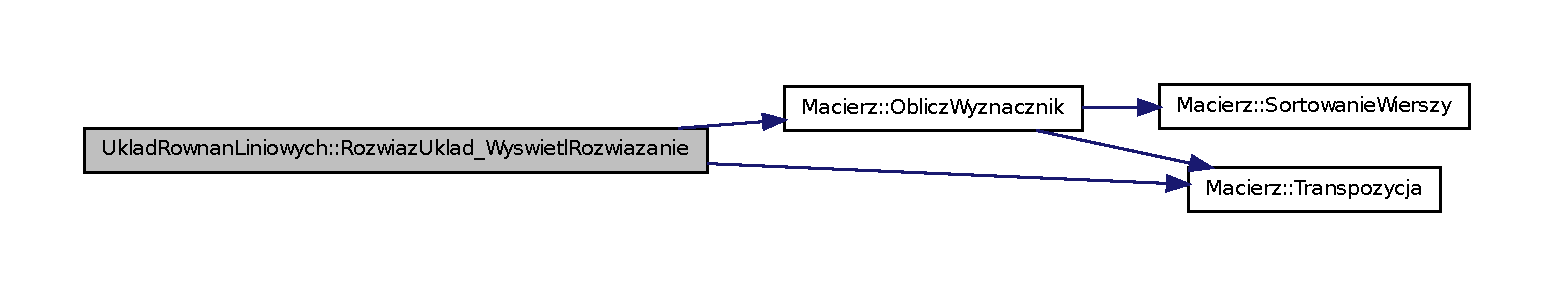
\includegraphics[width=400pt]{class_uklad_rownan_liniowych_a0d78de0a3797294e7d027d7791349637_cgraph}
\end{center}
\end{figure}




\subsection{Dokumentacja przyjaciół i funkcji związanych}
\hypertarget{class_uklad_rownan_liniowych_abf2a11f9dfab38690e476c7243a1c95d}{
\index{UkladRownanLiniowych@{UkladRownanLiniowych}!operator$<$$<$@{operator$<$$<$}}
\index{operator$<$$<$@{operator$<$$<$}!UkladRownanLiniowych@{UkladRownanLiniowych}}
\subsubsection[{operator$<$$<$}]{\setlength{\rightskip}{0pt plus 5cm}template$<$typename Typ, int ROZMIAR$>$ template$<$typename T , int rozmiarek$>$ std::ostream\& operator$<$$<$ (
\begin{DoxyParamCaption}
\item[{std::ostream \&}]{ Strm, }
\item[{const {\bf UkladRownanLiniowych}$<$ T, rozmiarek $>$ \&}]{ UklRown}
\end{DoxyParamCaption}
)\hspace{0.3cm}{\ttfamily  \mbox{[}friend\mbox{]}}}}
\label{class_uklad_rownan_liniowych_abf2a11f9dfab38690e476c7243a1c95d}
\hypertarget{class_uklad_rownan_liniowych_a5e3f1731c16e7f2a693237da0429dbb1}{
\index{UkladRownanLiniowych@{UkladRownanLiniowych}!operator$>$$>$@{operator$>$$>$}}
\index{operator$>$$>$@{operator$>$$>$}!UkladRownanLiniowych@{UkladRownanLiniowych}}
\subsubsection[{operator$>$$>$}]{\setlength{\rightskip}{0pt plus 5cm}template$<$typename Typ, int ROZMIAR$>$ template$<$typename T , int rozmiarek$>$ std::istream\& operator$>$$>$ (
\begin{DoxyParamCaption}
\item[{std::istream \&}]{ Strm, }
\item[{{\bf UkladRownanLiniowych}$<$ T, rozmiarek $>$ \&}]{ UklRown}
\end{DoxyParamCaption}
)\hspace{0.3cm}{\ttfamily  \mbox{[}friend\mbox{]}}}}
\label{class_uklad_rownan_liniowych_a5e3f1731c16e7f2a693237da0429dbb1}


\subsection{Dokumentacja atrybutów składowych}
\hypertarget{class_uklad_rownan_liniowych_a7fc31fd6f0dde9d7b95f136576af9471}{
\index{UkladRownanLiniowych@{UkladRownanLiniowych}!Mac@{Mac}}
\index{Mac@{Mac}!UkladRownanLiniowych@{UkladRownanLiniowych}}
\subsubsection[{Mac}]{\setlength{\rightskip}{0pt plus 5cm}template$<$typename Typ, int ROZMIAR$>$ {\bf Macierz}$<$Typ,ROZMIAR$>$ {\bf UkladRownanLiniowych}$<$ Typ, ROZMIAR $>$::{\bf Mac}\hspace{0.3cm}{\ttfamily  \mbox{[}private\mbox{]}}}}
\label{class_uklad_rownan_liniowych_a7fc31fd6f0dde9d7b95f136576af9471}


Definicja w linii 18 pliku UkladRownanLiniowych.hh.

\hypertarget{class_uklad_rownan_liniowych_ad6f84eeebcec882a5755868e05395486}{
\index{UkladRownanLiniowych@{UkladRownanLiniowych}!WyrazyWolne@{WyrazyWolne}}
\index{WyrazyWolne@{WyrazyWolne}!UkladRownanLiniowych@{UkladRownanLiniowych}}
\subsubsection[{WyrazyWolne}]{\setlength{\rightskip}{0pt plus 5cm}template$<$typename Typ, int ROZMIAR$>$ {\bf Wektor}$<$Typ,ROZMIAR$>$ {\bf UkladRownanLiniowych}$<$ Typ, ROZMIAR $>$::{\bf WyrazyWolne}\hspace{0.3cm}{\ttfamily  \mbox{[}private\mbox{]}}}}
\label{class_uklad_rownan_liniowych_ad6f84eeebcec882a5755868e05395486}


Definicja w linii 19 pliku UkladRownanLiniowych.hh.



Dokumentacja dla tej klasy została wygenerowana z pliku:\begin{DoxyCompactItemize}
\item 
\hyperlink{_uklad_rownan_liniowych_8hh}{UkladRownanLiniowych.hh}\end{DoxyCompactItemize}

\hypertarget{class_wektor}{
\section{Dokumentacja szablonu klasy Wektor$<$ Typ, ROZMIAR $>$}
\label{class_wektor}\index{Wektor@{Wektor}}
}


{\ttfamily \#include $<$Wektor.hh$>$}

\subsection*{Metody publiczne}
\begin{DoxyCompactItemize}
\item 
Typ \hyperlink{class_wektor_a0da276143fa53c457a7d1c836fe0fee6}{operator\mbox{[}$\,$\mbox{]}} (int Ind) const 
\begin{DoxyCompactList}\small\item\em Przeciazenia indeksow dla wektora Funkcja operatorowa \mbox{[}\mbox{]} sluzy do indeksowania klasy \hyperlink{class_wektor}{Wektor},by moc odnosic sie w bezposredni sposob do tablicy typu double tej klasy. \item\end{DoxyCompactList}\item 
Typ \& \hyperlink{class_wektor_ab1cf35ef42f4d254639df879b86560b5}{operator\mbox{[}$\,$\mbox{]}} (int Ind)
\begin{DoxyCompactList}\small\item\em Przeciazenia indeksow dla wektora Funkcja operatorowa \mbox{[}\mbox{]} sluzy do indeksowania klasy \hyperlink{class_wektor}{Wektor},by moc odnosic sie w bezposredni sposob do tablicy typu double tej klasy. \item\end{DoxyCompactList}\item 
\hyperlink{class_wektor}{Wektor}$<$ Typ, ROZMIAR $>$ \hyperlink{class_wektor_a69adce9a9015aa4ccca6320ca93a7a41}{operator$\ast$} (double liczba) const 
\begin{DoxyCompactList}\small\item\em Szablon funkcji operatorowej $\ast$ sluzy do mnozenia wektora przez liczbe. \item\end{DoxyCompactList}\item 
\hyperlink{class_wektor}{Wektor}$<$ Typ, ROZMIAR $>$ \hyperlink{class_wektor_a3dac94ec81b3bdbcd64565c3ae75230f}{operator+} (\hyperlink{class_wektor}{Wektor}$<$ Typ, ROZMIAR $>$ Q) const 
\begin{DoxyCompactList}\small\item\em Szablon funkcji operatorowej + sluzy do dodawania dwoch wektorow. \item\end{DoxyCompactList}\item 
\hyperlink{class_wektor}{Wektor}$<$ Typ, ROZMIAR $>$ \hyperlink{class_wektor_a369fcd56f09fe24c09582ab65f737cbf}{operator-\/} (\hyperlink{class_wektor}{Wektor}$<$ Typ, ROZMIAR $>$ Q) const 
\begin{DoxyCompactList}\small\item\em Szablon Funkcji operatorowej -\/ sluzy do odejmowania dwoch wektorow. \item\end{DoxyCompactList}\item 
\hyperlink{class_wektor}{Wektor}$<$ Typ, ROZMIAR $>$ \hyperlink{class_wektor_aa0e6e381f2099b4b6c8a0131e2c2f6e4}{operator/} (double Liczba) const 
\begin{DoxyCompactList}\small\item\em Szablon funkcji operatorowej / sluzy do dzielenia wektora przez liczbe. \item\end{DoxyCompactList}\item 
Typ \hyperlink{class_wektor_a4ef2829992c2337f21c78e36b3b08cb8}{operator$\ast$} (\hyperlink{class_wektor}{Wektor}$<$ Typ, ROZMIAR $>$ Q) const 
\begin{DoxyCompactList}\small\item\em Szablon funkcji operatorowej $\ast$ sluzy do mnozenia wektor przez wektor. \item\end{DoxyCompactList}\end{DoxyCompactItemize}
\subsection*{Atrybuty prywatne}
\begin{DoxyCompactItemize}
\item 
Typ \hyperlink{class_wektor_a0d996feb5ea3412a985abaac93060e4b}{\_\-V} \mbox{[}ROZMIAR\mbox{]}
\end{DoxyCompactItemize}
\subsection*{Przyjaciele}
\begin{DoxyCompactItemize}
\item 
{\footnotesize template$<$typename T , int rozmiarek$>$ }\\\hyperlink{class_wektor}{Wektor}$<$ T, rozmiarek $>$ \hyperlink{class_wektor_a2ac81a8a61e14506afca4629675977af}{operator$\ast$} (const double Liczba, const \hyperlink{class_wektor}{Wektor}$<$ T, rozmiarek $>$ \hyperlink{class_wektor_a0d996feb5ea3412a985abaac93060e4b}{\_\-V})
\begin{DoxyCompactList}\small\item\em Szablon funkcji operatorowej $\ast$ sluzy do mnozenia liczby przez wektor. \item\end{DoxyCompactList}\end{DoxyCompactItemize}


\subsection{Opis szczegółowy}
\subsubsection*{template$<$typename Typ, int ROZMIAR$>$ class Wektor$<$ Typ, ROZMIAR $>$}



Definicja w linii 14 pliku Wektor.hh.



\subsection{Dokumentacja funkcji składowych}
\hypertarget{class_wektor_a69adce9a9015aa4ccca6320ca93a7a41}{
\index{Wektor@{Wektor}!operator$\ast$@{operator$\ast$}}
\index{operator$\ast$@{operator$\ast$}!Wektor@{Wektor}}
\subsubsection[{operator$\ast$}]{\setlength{\rightskip}{0pt plus 5cm}template$<$typename Typ , int ROZMIAR$>$ {\bf Wektor}$<$ Typ, ROZMIAR $>$ {\bf Wektor}$<$ Typ, ROZMIAR $>$::operator$\ast$ (
\begin{DoxyParamCaption}
\item[{double}]{ Liczba}
\end{DoxyParamCaption}
) const}}
\label{class_wektor_a69adce9a9015aa4ccca6320ca93a7a41}
\begin{DoxyReturn}{Zwraca}
element typu \hyperlink{class_wektor}{Wektor} 
\end{DoxyReturn}

\begin{DoxyParams}{Parametry}
\item[{\em Liczba-\/}]liczba rzeczywista \end{DoxyParams}
\begin{DoxyPrecond}{Warunek wstępny}
poprawne wczytanie wektora i podanie liczby 
\end{DoxyPrecond}
\begin{DoxyReturn}{Zwraca}
mnozenie wektora przw wektor, wartosc zwracana przez funkcje 
\end{DoxyReturn}


Definicja w linii 105 pliku Wektor.hh.

\hypertarget{class_wektor_a4ef2829992c2337f21c78e36b3b08cb8}{
\index{Wektor@{Wektor}!operator$\ast$@{operator$\ast$}}
\index{operator$\ast$@{operator$\ast$}!Wektor@{Wektor}}
\subsubsection[{operator$\ast$}]{\setlength{\rightskip}{0pt plus 5cm}template$<$typename Typ , int ROZMIAR$>$ Typ {\bf Wektor}$<$ Typ, ROZMIAR $>$::operator$\ast$ (
\begin{DoxyParamCaption}
\item[{{\bf Wektor}$<$ Typ, ROZMIAR $>$}]{ Q}
\end{DoxyParamCaption}
) const}}
\label{class_wektor_a4ef2829992c2337f21c78e36b3b08cb8}
\begin{DoxyReturn}{Zwraca}
element typu double 
\end{DoxyReturn}

\begin{DoxyParams}{Parametry}
\item[\mbox{\tt[in]} {\em Q-\/}]element typu szablon wektor \end{DoxyParams}
\begin{DoxyPrecond}{Warunek wstępny}
poprawne wczytanie 2 wektorow 
\end{DoxyPrecond}
\begin{DoxyReturn}{Zwraca}
mnozenie wektora przez wektor, wynik jako wartosc zwracana przez funkcje 
\end{DoxyReturn}


Definicja w linii 136 pliku Wektor.hh.

\hypertarget{class_wektor_a3dac94ec81b3bdbcd64565c3ae75230f}{
\index{Wektor@{Wektor}!operator+@{operator+}}
\index{operator+@{operator+}!Wektor@{Wektor}}
\subsubsection[{operator+}]{\setlength{\rightskip}{0pt plus 5cm}template$<$typename Typ , int ROZMIAR$>$ {\bf Wektor}$<$ Typ, ROZMIAR $>$ {\bf Wektor}$<$ Typ, ROZMIAR $>$::operator+ (
\begin{DoxyParamCaption}
\item[{{\bf Wektor}$<$ Typ, ROZMIAR $>$}]{ Q}
\end{DoxyParamCaption}
) const}}
\label{class_wektor_a3dac94ec81b3bdbcd64565c3ae75230f}
\begin{DoxyReturn}{Zwraca}
referencja \hyperlink{class_wektor}{Wektor} 
\end{DoxyReturn}

\begin{DoxyParams}{Parametry}
\item[\mbox{\tt[in]} {\em Q}]-\/ argument typu szablon \hyperlink{class_wektor}{Wektor} \end{DoxyParams}
\begin{DoxyPrecond}{Warunek wstępny}
poprawne wczytanie dwoch wektorow 
\end{DoxyPrecond}
\begin{DoxyReturn}{Zwraca}
dodanie dwoch wektorow, wynik jako wartosc zwracana przez funkcje 
\end{DoxyReturn}


Definicja w linii 152 pliku Wektor.hh.

\hypertarget{class_wektor_a369fcd56f09fe24c09582ab65f737cbf}{
\index{Wektor@{Wektor}!operator-\/@{operator-\/}}
\index{operator-\/@{operator-\/}!Wektor@{Wektor}}
\subsubsection[{operator-\/}]{\setlength{\rightskip}{0pt plus 5cm}template$<$typename Typ , int ROZMIAR$>$ {\bf Wektor}$<$ Typ, ROZMIAR $>$ {\bf Wektor}$<$ Typ, ROZMIAR $>$::operator-\/ (
\begin{DoxyParamCaption}
\item[{{\bf Wektor}$<$ Typ, ROZMIAR $>$}]{ Q}
\end{DoxyParamCaption}
) const}}
\label{class_wektor_a369fcd56f09fe24c09582ab65f737cbf}
\begin{DoxyReturn}{Zwraca}
referencja do \hyperlink{class_wektor}{Wektor} 
\end{DoxyReturn}

\begin{DoxyParams}{Parametry}
\item[\mbox{\tt[in]} {\em Q}]-\/ argument typu szablon \hyperlink{class_wektor}{Wektor} \end{DoxyParams}
\begin{DoxyPrecond}{Warunek wstępny}
poprawne wczytanie dwoch wektorow 
\end{DoxyPrecond}
\begin{DoxyReturn}{Zwraca}
odjecie dwoch wektorow, wynik jako wartosc zwracana przez funkcje 
\end{DoxyReturn}


Definicja w linii 167 pliku Wektor.hh.

\hypertarget{class_wektor_aa0e6e381f2099b4b6c8a0131e2c2f6e4}{
\index{Wektor@{Wektor}!operator/@{operator/}}
\index{operator/@{operator/}!Wektor@{Wektor}}
\subsubsection[{operator/}]{\setlength{\rightskip}{0pt plus 5cm}template$<$typename Typ , int ROZMIAR$>$ {\bf Wektor}$<$ Typ, ROZMIAR $>$ {\bf Wektor}$<$ Typ, ROZMIAR $>$::operator/ (
\begin{DoxyParamCaption}
\item[{double}]{ Liczba}
\end{DoxyParamCaption}
) const}}
\label{class_wektor_aa0e6e381f2099b4b6c8a0131e2c2f6e4}
\begin{DoxyReturn}{Zwraca}
referencja \hyperlink{class_wektor}{Wektor} 
\end{DoxyReturn}

\begin{DoxyParams}{Parametry}
\item[\mbox{\tt[in]} {\em Liczba}]-\/ liczba rzeczywista \end{DoxyParams}
\begin{DoxyPrecond}{Warunek wstępny}
poprawne wczytanie wektora i podanie liczby 
\end{DoxyPrecond}
\begin{DoxyReturn}{Zwraca}
dzielenie wektora przez liczbe, wynik jako wartosc zwracana przez funkcje 
\end{DoxyReturn}


Definicja w linii 182 pliku Wektor.hh.

\hypertarget{class_wektor_ab1cf35ef42f4d254639df879b86560b5}{
\index{Wektor@{Wektor}!operator\mbox{[}\mbox{]}@{operator[]}}
\index{operator\mbox{[}\mbox{]}@{operator[]}!Wektor@{Wektor}}
\subsubsection[{operator[]}]{\setlength{\rightskip}{0pt plus 5cm}template$<$typename Typ, int ROZMIAR$>$ Typ\& {\bf Wektor}$<$ Typ, ROZMIAR $>$::operator\mbox{[}$\,$\mbox{]} (
\begin{DoxyParamCaption}
\item[{int}]{ Ind}
\end{DoxyParamCaption}
)\hspace{0.3cm}{\ttfamily  \mbox{[}inline\mbox{]}}}}
\label{class_wektor_ab1cf35ef42f4d254639df879b86560b5}
\begin{DoxyPrecond}{Warunek wstępny}
poprawny argument(int) w indeksie 
\end{DoxyPrecond}
\begin{DoxyReturn}{Zwraca}
wynik,jako wartosc double zwracana przez funkcje 
\end{DoxyReturn}


Definicja w linii 35 pliku Wektor.hh.

\hypertarget{class_wektor_a0da276143fa53c457a7d1c836fe0fee6}{
\index{Wektor@{Wektor}!operator\mbox{[}\mbox{]}@{operator[]}}
\index{operator\mbox{[}\mbox{]}@{operator[]}!Wektor@{Wektor}}
\subsubsection[{operator[]}]{\setlength{\rightskip}{0pt plus 5cm}template$<$typename Typ, int ROZMIAR$>$ Typ {\bf Wektor}$<$ Typ, ROZMIAR $>$::operator\mbox{[}$\,$\mbox{]} (
\begin{DoxyParamCaption}
\item[{int}]{ Ind}
\end{DoxyParamCaption}
) const\hspace{0.3cm}{\ttfamily  \mbox{[}inline\mbox{]}}}}
\label{class_wektor_a0da276143fa53c457a7d1c836fe0fee6}
\begin{DoxyPrecond}{Warunek wstępny}
poprawny argument(int) w indeksie 
\end{DoxyPrecond}
\begin{DoxyReturn}{Zwraca}
wynik,jako wartosc double zwracana przez funkcje 
\end{DoxyReturn}


Definicja w linii 26 pliku Wektor.hh.



\subsection{Dokumentacja przyjaciół i funkcji związanych}
\hypertarget{class_wektor_a2ac81a8a61e14506afca4629675977af}{
\index{Wektor@{Wektor}!operator$\ast$@{operator$\ast$}}
\index{operator$\ast$@{operator$\ast$}!Wektor@{Wektor}}
\subsubsection[{operator$\ast$}]{\setlength{\rightskip}{0pt plus 5cm}template$<$typename Typ, int ROZMIAR$>$ template$<$typename T , int rozmiarek$>$ {\bf Wektor}$<$T,rozmiarek$>$ operator$\ast$ (
\begin{DoxyParamCaption}
\item[{const double}]{ Liczba, }
\item[{const {\bf Wektor}$<$ T, rozmiarek $>$}]{ \_\-V}
\end{DoxyParamCaption}
)\hspace{0.3cm}{\ttfamily  \mbox{[}friend\mbox{]}}}}
\label{class_wektor_a2ac81a8a61e14506afca4629675977af}


\subsection{Dokumentacja atrybutów składowych}
\hypertarget{class_wektor_a0d996feb5ea3412a985abaac93060e4b}{
\index{Wektor@{Wektor}!\_\-V@{\_\-V}}
\index{\_\-V@{\_\-V}!Wektor@{Wektor}}
\subsubsection[{\_\-V}]{\setlength{\rightskip}{0pt plus 5cm}template$<$typename Typ, int ROZMIAR$>$ Typ {\bf Wektor}$<$ Typ, ROZMIAR $>$::{\bf \_\-V}\mbox{[}ROZMIAR\mbox{]}\hspace{0.3cm}{\ttfamily  \mbox{[}private\mbox{]}}}}
\label{class_wektor_a0d996feb5ea3412a985abaac93060e4b}


Definicja w linii 15 pliku Wektor.hh.



Dokumentacja dla tej klasy została wygenerowana z pliku:\begin{DoxyCompactItemize}
\item 
\hyperlink{_wektor_8hh}{Wektor.hh}\end{DoxyCompactItemize}

\chapter{Dokumentacja plików}
\hypertarget{_l_zespolona_8cpp}{
\section{Dokumentacja pliku LZespolona.cpp}
\label{_l_zespolona_8cpp}\index{LZespolona.cpp@{LZespolona.cpp}}
}


Definicja metod klasy LZesp.  


{\ttfamily \#include $<$cmath$>$}\par
{\ttfamily \#include $<$iostream$>$}\par
{\ttfamily \#include $<$cstdlib$>$}\par
{\ttfamily \#include \char`\"{}LZespolona.hh\char`\"{}}\par
Wykres zależności załączania dla LZespolona.cpp:\nopagebreak
\begin{figure}[H]
\begin{center}
\leavevmode
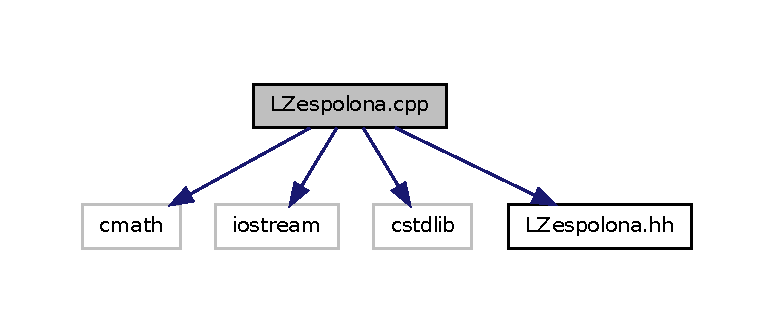
\includegraphics[width=372pt]{_l_zespolona_8cpp__incl}
\end{center}
\end{figure}
\subsection*{Funkcje}
\begin{DoxyCompactItemize}
\item 
\hyperlink{class_l_zespolona}{LZespolona} \hyperlink{_l_zespolona_8cpp_a48f8e9c2b37ad5b3b8b964c25346b930}{operator+} (const double Liczba, const \hyperlink{class_l_zespolona}{LZespolona} \&Z)
\begin{DoxyCompactList}\small\item\em Funkcja operatorowa dodaje liczbe rzeczywista do liczby zespolonej. \item\end{DoxyCompactList}\item 
\hyperlink{class_l_zespolona}{LZespolona} \hyperlink{_l_zespolona_8cpp_aef47f3e429efa18ade4555f77df27014}{operator+} (const \hyperlink{class_l_zespolona}{LZespolona} \&Z, const double Liczba)
\begin{DoxyCompactList}\small\item\em Funkcja operatorowa dodaje liczbe rzeczywista do liczby zespolonej. \item\end{DoxyCompactList}\item 
\hyperlink{class_l_zespolona}{LZespolona} \hyperlink{_l_zespolona_8cpp_afd6ac9993dc5c5279a990b98d607b2d4}{operator-\/} (const \hyperlink{class_l_zespolona}{LZespolona} \&Z, const double Liczba)
\begin{DoxyCompactList}\small\item\em Funkcja operatorowa odejmuje liczbe rzeczywista od liczby zespolonej. \item\end{DoxyCompactList}\item 
\hyperlink{class_l_zespolona}{LZespolona} \hyperlink{_l_zespolona_8cpp_a896efd2b35c96235e487819ad646aebb}{operator$\ast$} (const double Liczba, const \hyperlink{class_l_zespolona}{LZespolona} \&Z)
\begin{DoxyCompactList}\small\item\em Funkcja operatorowa mnozy liczbe rzeczywista do liczby zespolonej. \item\end{DoxyCompactList}\item 
\hyperlink{class_l_zespolona}{LZespolona} \hyperlink{_l_zespolona_8cpp_a7cc8baeda5b16a42f0a193d3fbaf0a64}{operator$\ast$} (const \hyperlink{class_l_zespolona}{LZespolona} \&Z, const double Liczba)
\begin{DoxyCompactList}\small\item\em Funkcja operatorowa mnozy liczbe rzeczywista do liczby zespolonej. \item\end{DoxyCompactList}\item 
\hyperlink{class_l_zespolona}{LZespolona} \hyperlink{_l_zespolona_8cpp_adde8e8baef5452a13cc50c8c72e8d397}{operator/} (const \hyperlink{class_l_zespolona}{LZespolona} \&Z, const double Liczba)
\begin{DoxyCompactList}\small\item\em Funkcja operatorowa dzieli liczbe zespolona przez liczbe zespolona. \item\end{DoxyCompactList}\item 
std::ostream \& \hyperlink{_l_zespolona_8cpp_ab7b96610b555631a2b10bd9c097abb55}{operator$<$$<$} (std::ostream \&Strm, const \hyperlink{class_l_zespolona}{LZespolona} \&WyswLiczba)
\begin{DoxyCompactList}\small\item\em Funkcja operatorowa pozwala na wypisanie liczby zespolonej. \item\end{DoxyCompactList}\item 
std::istream \& \hyperlink{_l_zespolona_8cpp_a36c8f5a74b4b81f5c1f9142ad5a958b9}{operator$>$$>$} (std::istream \&Strm, \hyperlink{class_l_zespolona}{LZespolona} \&Z)
\begin{DoxyCompactList}\small\item\em Funkcja operatorowa pozwala na wczytanie liczby zespolonej. \item\end{DoxyCompactList}\end{DoxyCompactItemize}


\subsection{Opis szczegółowy}
Zawiera definicje metod klasy LZesp. 

Definicja w pliku \hyperlink{_l_zespolona_8cpp_source}{LZespolona.cpp}.



\subsection{Dokumentacja funkcji}
\hypertarget{_l_zespolona_8cpp_a896efd2b35c96235e487819ad646aebb}{
\index{LZespolona.cpp@{LZespolona.cpp}!operator$\ast$@{operator$\ast$}}
\index{operator$\ast$@{operator$\ast$}!LZespolona.cpp@{LZespolona.cpp}}
\subsubsection[{operator$\ast$}]{\setlength{\rightskip}{0pt plus 5cm}{\bf LZespolona} operator$\ast$ (
\begin{DoxyParamCaption}
\item[{const double}]{ Liczba, }
\item[{const {\bf LZespolona} \&}]{ Z}
\end{DoxyParamCaption}
)}}
\label{_l_zespolona_8cpp_a896efd2b35c96235e487819ad646aebb}

\begin{DoxyParams}{Parametry}
\item[{\em Z}]-\/ liczba zespolona. \item[{\em Liczba}]-\/ liczba rzeczywista \end{DoxyParams}
\begin{DoxyReturn}{Zwraca}
Zwraca liczbe zespolona. 
\end{DoxyReturn}
\begin{DoxyPrecond}{Warunek wstępny}
Poprawne wczytanie dwoch liczb zespolonych 
\end{DoxyPrecond}


Definicja w linii 158 pliku LZespolona.cpp.

\hypertarget{_l_zespolona_8cpp_a7cc8baeda5b16a42f0a193d3fbaf0a64}{
\index{LZespolona.cpp@{LZespolona.cpp}!operator$\ast$@{operator$\ast$}}
\index{operator$\ast$@{operator$\ast$}!LZespolona.cpp@{LZespolona.cpp}}
\subsubsection[{operator$\ast$}]{\setlength{\rightskip}{0pt plus 5cm}{\bf LZespolona} operator$\ast$ (
\begin{DoxyParamCaption}
\item[{const {\bf LZespolona} \&}]{ Z, }
\item[{const double}]{ Liczba}
\end{DoxyParamCaption}
)}}
\label{_l_zespolona_8cpp_a7cc8baeda5b16a42f0a193d3fbaf0a64}

\begin{DoxyParams}{Parametry}
\item[{\em Z}]-\/ liczba zespolona. \item[{\em Liczba}]-\/ liczba rzeczywista \end{DoxyParams}
\begin{DoxyReturn}{Zwraca}
Zwraca liczbe zespolona. 
\end{DoxyReturn}
\begin{DoxyPrecond}{Warunek wstępny}
Poprawne wczytanie dwoch liczb zespolonych 
\end{DoxyPrecond}


Definicja w linii 174 pliku LZespolona.cpp.

\hypertarget{_l_zespolona_8cpp_aef47f3e429efa18ade4555f77df27014}{
\index{LZespolona.cpp@{LZespolona.cpp}!operator+@{operator+}}
\index{operator+@{operator+}!LZespolona.cpp@{LZespolona.cpp}}
\subsubsection[{operator+}]{\setlength{\rightskip}{0pt plus 5cm}{\bf LZespolona} operator+ (
\begin{DoxyParamCaption}
\item[{const {\bf LZespolona} \&}]{ Z, }
\item[{const double}]{ Liczba}
\end{DoxyParamCaption}
)}}
\label{_l_zespolona_8cpp_aef47f3e429efa18ade4555f77df27014}

\begin{DoxyParams}{Parametry}
\item[{\em Z}]-\/ liczba zespolona. \item[{\em Liczba}]-\/ liczba rzeczywista \end{DoxyParams}
\begin{DoxyReturn}{Zwraca}
Zwraca liczbe zespolona. 
\end{DoxyReturn}
\begin{DoxyPrecond}{Warunek wstępny}
Poprawne wczytanie dwoch liczb zespolonych 
\end{DoxyPrecond}


Definicja w linii 128 pliku LZespolona.cpp.

\hypertarget{_l_zespolona_8cpp_a48f8e9c2b37ad5b3b8b964c25346b930}{
\index{LZespolona.cpp@{LZespolona.cpp}!operator+@{operator+}}
\index{operator+@{operator+}!LZespolona.cpp@{LZespolona.cpp}}
\subsubsection[{operator+}]{\setlength{\rightskip}{0pt plus 5cm}{\bf LZespolona} operator+ (
\begin{DoxyParamCaption}
\item[{const double}]{ Liczba, }
\item[{const {\bf LZespolona} \&}]{ Z}
\end{DoxyParamCaption}
)}}
\label{_l_zespolona_8cpp_a48f8e9c2b37ad5b3b8b964c25346b930}

\begin{DoxyParams}{Parametry}
\item[{\em Z}]-\/ liczba zespolona. \item[{\em Liczba}]-\/ liczba rzeczywista \end{DoxyParams}
\begin{DoxyReturn}{Zwraca}
Zwraca liczbe zespolona. 
\end{DoxyReturn}
\begin{DoxyPrecond}{Warunek wstępny}
Poprawne wczytanie dwoch liczb zespolonych 
\end{DoxyPrecond}


Definicja w linii 113 pliku LZespolona.cpp.

\hypertarget{_l_zespolona_8cpp_afd6ac9993dc5c5279a990b98d607b2d4}{
\index{LZespolona.cpp@{LZespolona.cpp}!operator-\/@{operator-\/}}
\index{operator-\/@{operator-\/}!LZespolona.cpp@{LZespolona.cpp}}
\subsubsection[{operator-\/}]{\setlength{\rightskip}{0pt plus 5cm}{\bf LZespolona} operator-\/ (
\begin{DoxyParamCaption}
\item[{const {\bf LZespolona} \&}]{ Z, }
\item[{const double}]{ Liczba}
\end{DoxyParamCaption}
)}}
\label{_l_zespolona_8cpp_afd6ac9993dc5c5279a990b98d607b2d4}

\begin{DoxyParams}{Parametry}
\item[{\em Z}]-\/ liczba zespolona. \item[{\em Liczba}]-\/ liczba rzeczywista \end{DoxyParams}
\begin{DoxyReturn}{Zwraca}
Zwraca liczbe zespolona. 
\end{DoxyReturn}
\begin{DoxyPrecond}{Warunek wstępny}
Poprawne wczytanie dwoch liczb zespolonych 
\end{DoxyPrecond}


Definicja w linii 143 pliku LZespolona.cpp.

\hypertarget{_l_zespolona_8cpp_adde8e8baef5452a13cc50c8c72e8d397}{
\index{LZespolona.cpp@{LZespolona.cpp}!operator/@{operator/}}
\index{operator/@{operator/}!LZespolona.cpp@{LZespolona.cpp}}
\subsubsection[{operator/}]{\setlength{\rightskip}{0pt plus 5cm}{\bf LZespolona} operator/ (
\begin{DoxyParamCaption}
\item[{const {\bf LZespolona} \&}]{ Z, }
\item[{const double}]{ Liczba}
\end{DoxyParamCaption}
)}}
\label{_l_zespolona_8cpp_adde8e8baef5452a13cc50c8c72e8d397}

\begin{DoxyParams}{Parametry}
\item[{\em Z}]-\/ liczba zespolona. \item[{\em Liczba}]-\/ liczba rzeczywista \end{DoxyParams}
\begin{DoxyReturn}{Zwraca}
Zwraca liczbe zespolona. 
\end{DoxyReturn}
\begin{DoxyPrecond}{Warunek wstępny}
Poprawne wczytanie dwoch liczb zespolonych 
\end{DoxyPrecond}


Definicja w linii 190 pliku LZespolona.cpp.

\hypertarget{_l_zespolona_8cpp_ab7b96610b555631a2b10bd9c097abb55}{
\index{LZespolona.cpp@{LZespolona.cpp}!operator$<$$<$@{operator$<$$<$}}
\index{operator$<$$<$@{operator$<$$<$}!LZespolona.cpp@{LZespolona.cpp}}
\subsubsection[{operator$<$$<$}]{\setlength{\rightskip}{0pt plus 5cm}std::ostream\& operator$<$$<$ (
\begin{DoxyParamCaption}
\item[{std::ostream \&}]{ Strm, }
\item[{const {\bf LZespolona} \&}]{ WyswLiczba}
\end{DoxyParamCaption}
)}}
\label{_l_zespolona_8cpp_ab7b96610b555631a2b10bd9c097abb55}

\begin{DoxyParams}{Parametry}
\item[\mbox{\tt[in,out]} {\em \&Strm}]-\/ referencja do strumienia wyjsciowego \item[\mbox{\tt[in,out]} {\em \&WyswLiczba}]refencja do klasy typu LZesp \end{DoxyParams}
\begin{DoxyReturn}{Zwraca}
Zwraca referencje do strumienia wyjsciowego 
\end{DoxyReturn}
\begin{DoxyPrecond}{Warunek wstępny}
Poprawne wczytanie liczby zespolonej 
\end{DoxyPrecond}


Definicja w linii 205 pliku LZespolona.cpp.

\hypertarget{_l_zespolona_8cpp_a36c8f5a74b4b81f5c1f9142ad5a958b9}{
\index{LZespolona.cpp@{LZespolona.cpp}!operator$>$$>$@{operator$>$$>$}}
\index{operator$>$$>$@{operator$>$$>$}!LZespolona.cpp@{LZespolona.cpp}}
\subsubsection[{operator$>$$>$}]{\setlength{\rightskip}{0pt plus 5cm}std::istream\& operator$>$$>$ (
\begin{DoxyParamCaption}
\item[{std::istream \&}]{ Strm, }
\item[{{\bf LZespolona} \&}]{ Z}
\end{DoxyParamCaption}
)}}
\label{_l_zespolona_8cpp_a36c8f5a74b4b81f5c1f9142ad5a958b9}

\begin{DoxyParams}{Parametry}
\item[\mbox{\tt[in,out]} {\em \&Strm}]-\/ referencja do strumienia wejsciowego \item[\mbox{\tt[in,out]} {\em \&Z}]referencja do klasy typu LZesp \end{DoxyParams}
\begin{DoxyReturn}{Zwraca}
Zwraca referencje do strumienia wejsciowego 
\end{DoxyReturn}
\begin{DoxyPrecond}{Warunek wstępny}
Liczbe nalezy podawac w nawiasach klamrowych 

Zawsze musi byc podana czesc rzeczywista i czesc urojona 
\end{DoxyPrecond}


Definicja w linii 245 pliku LZespolona.cpp.


\hypertarget{_l_zespolona_8hh}{
\section{Dokumentacja pliku LZespolona.hh}
\label{_l_zespolona_8hh}\index{LZespolona.hh@{LZespolona.hh}}
}


Klasa \hyperlink{class_l_zespolona}{LZespolona} sluzy do przechowywania liczby zespolonej w programie oraz do wykonywania operacji matematycznych na niej.  


Ten wykres pokazuje, które pliki bezpośrednio lub pośrednio załączają ten plik:\nopagebreak
\begin{figure}[H]
\begin{center}
\leavevmode
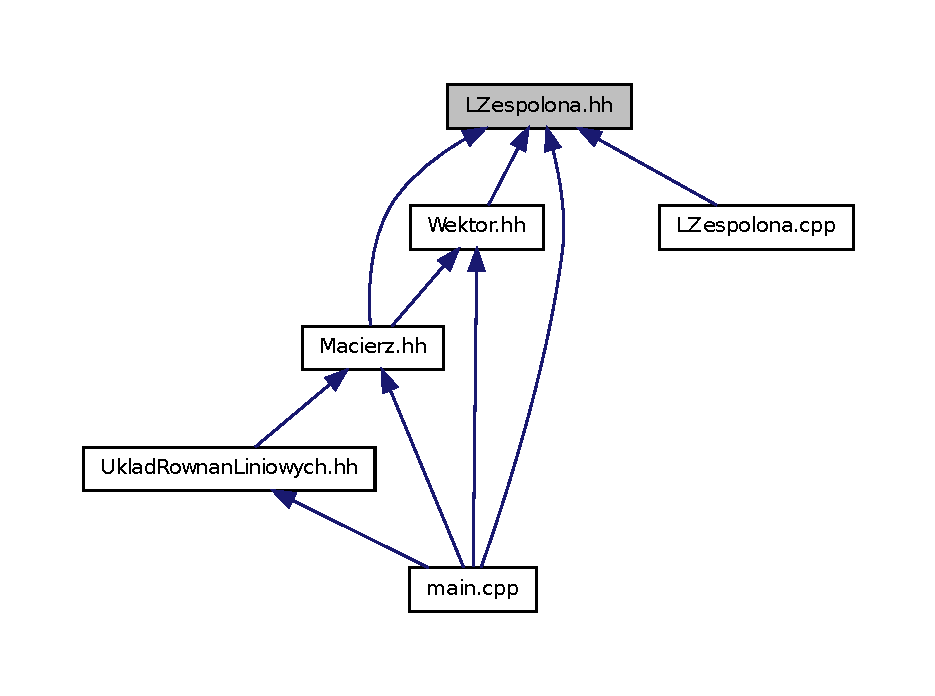
\includegraphics[width=400pt]{_l_zespolona_8hh__dep__incl}
\end{center}
\end{figure}
\subsection*{Komponenty}
\begin{DoxyCompactItemize}
\item 
class \hyperlink{class_l_zespolona}{LZespolona}
\end{DoxyCompactItemize}
\subsection*{Funkcje}
\begin{DoxyCompactItemize}
\item 
std::ostream \& \hyperlink{_l_zespolona_8hh_ab7b96610b555631a2b10bd9c097abb55}{operator$<$$<$} (std::ostream \&Strm, const \hyperlink{class_l_zespolona}{LZespolona} \&WyswLiczba)
\begin{DoxyCompactList}\small\item\em Funkcja operatorowa pozwala na wypisanie liczby zespolonej. \item\end{DoxyCompactList}\item 
std::istream \& \hyperlink{_l_zespolona_8hh_a36c8f5a74b4b81f5c1f9142ad5a958b9}{operator$>$$>$} (std::istream \&Strm, \hyperlink{class_l_zespolona}{LZespolona} \&Z)
\begin{DoxyCompactList}\small\item\em Funkcja operatorowa pozwala na wczytanie liczby zespolonej. \item\end{DoxyCompactList}\end{DoxyCompactItemize}


\subsection{Opis szczegółowy}


Definicja w pliku \hyperlink{_l_zespolona_8hh_source}{LZespolona.hh}.



\subsection{Dokumentacja funkcji}
\hypertarget{_l_zespolona_8hh_ab7b96610b555631a2b10bd9c097abb55}{
\index{LZespolona.hh@{LZespolona.hh}!operator$<$$<$@{operator$<$$<$}}
\index{operator$<$$<$@{operator$<$$<$}!LZespolona.hh@{LZespolona.hh}}
\subsubsection[{operator$<$$<$}]{\setlength{\rightskip}{0pt plus 5cm}std::ostream\& operator$<$$<$ (
\begin{DoxyParamCaption}
\item[{std::ostream \&}]{ Strm, }
\item[{const {\bf LZespolona} \&}]{ WyswLiczba}
\end{DoxyParamCaption}
)}}
\label{_l_zespolona_8hh_ab7b96610b555631a2b10bd9c097abb55}
brief Wyswietlenie liczby zespolonej


\begin{DoxyParams}{Parametry}
\item[\mbox{\tt[in,out]} {\em \&Strm}]-\/ referencja do strumienia wyjsciowego \item[\mbox{\tt[in,out]} {\em \&WyswLiczba}]refencja do klasy typu LZesp \end{DoxyParams}
\begin{DoxyReturn}{Zwraca}
Zwraca referencje do strumienia wyjsciowego 
\end{DoxyReturn}
\begin{DoxyPrecond}{Warunek wstępny}
Poprawne wczytanie liczby zespolonej 
\end{DoxyPrecond}


Definicja w linii 205 pliku LZespolona.cpp.

\hypertarget{_l_zespolona_8hh_a36c8f5a74b4b81f5c1f9142ad5a958b9}{
\index{LZespolona.hh@{LZespolona.hh}!operator$>$$>$@{operator$>$$>$}}
\index{operator$>$$>$@{operator$>$$>$}!LZespolona.hh@{LZespolona.hh}}
\subsubsection[{operator$>$$>$}]{\setlength{\rightskip}{0pt plus 5cm}std::istream\& operator$>$$>$ (
\begin{DoxyParamCaption}
\item[{std::istream \&}]{ Strm, }
\item[{{\bf LZespolona} \&}]{ Z}
\end{DoxyParamCaption}
)}}
\label{_l_zespolona_8hh_a36c8f5a74b4b81f5c1f9142ad5a958b9}
brief Wczytywanie liczby zespolonej


\begin{DoxyParams}{Parametry}
\item[\mbox{\tt[in,out]} {\em \&Strm}]-\/ referencja do strumienia wejsciowego \item[\mbox{\tt[in,out]} {\em \&Z}]referencja do klasy typu LZesp \end{DoxyParams}
\begin{DoxyReturn}{Zwraca}
Zwraca referencje do strumienia wejsciowego 
\end{DoxyReturn}
\begin{DoxyPrecond}{Warunek wstępny}
Liczbe nalezy podawac w nawiasach klamrowych 

Zawsze musi byc podana czesc rzeczywista i czesc urojona 
\end{DoxyPrecond}


Definicja w linii 245 pliku LZespolona.cpp.


\hypertarget{_macierz_8hh}{
\section{Dokumentacja pliku Macierz.hh}
\label{_macierz_8hh}\index{Macierz.hh@{Macierz.hh}}
}


Szablon Klasy \hyperlink{class_macierz}{Macierz} modeluje w programie macierz. \hyperlink{class_macierz}{Macierz} jest przechowywana w postaci Wektorow. Ich ilosc zalezy od rozmiaru Macierzy. Sklada sie z metody do obliczania wyznacznika i operatora indeksujacego,by bezposrednio odwolywac sie do macierzy. Sklada sie rowniez z funkcji arytmetycznych na macierzach.  


{\ttfamily \#include \char`\"{}Wektor.hh\char`\"{}}\par
{\ttfamily \#include $<$iostream$>$}\par
{\ttfamily \#include \char`\"{}LZespolona.hh\char`\"{}}\par
Wykres zależności załączania dla Macierz.hh:\nopagebreak
\begin{figure}[H]
\begin{center}
\leavevmode
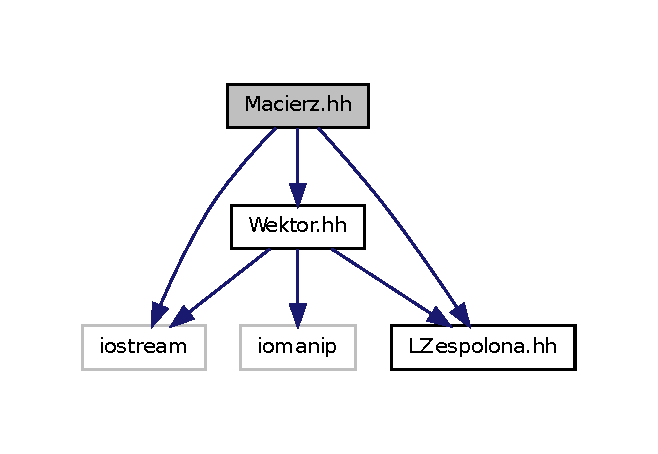
\includegraphics[width=316pt]{_macierz_8hh__incl}
\end{center}
\end{figure}
Ten wykres pokazuje, które pliki bezpośrednio lub pośrednio załączają ten plik:\nopagebreak
\begin{figure}[H]
\begin{center}
\leavevmode
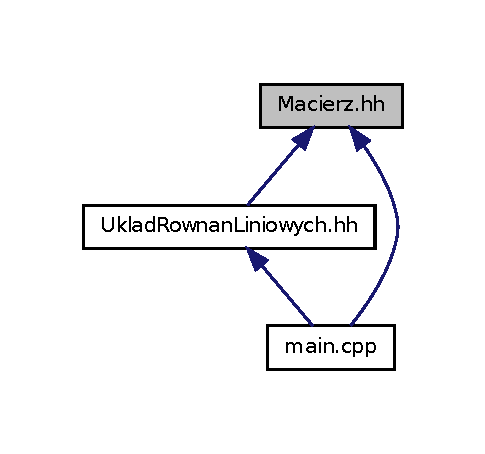
\includegraphics[width=233pt]{_macierz_8hh__dep__incl}
\end{center}
\end{figure}
\subsection*{Komponenty}
\begin{DoxyCompactItemize}
\item 
class \hyperlink{class_macierz}{Macierz$<$ Typ, ROZMIAR $>$}
\end{DoxyCompactItemize}
\subsection*{Funkcje}
\begin{DoxyCompactItemize}
\item 
{\footnotesize template$<$typename Typ , int ROZMIAR$>$ }\\istream \& \hyperlink{_macierz_8hh_a1c08e6a33bb216fa9634ec5dc037d2fa}{operator$>$$>$} (istream \&Strm, \hyperlink{class_macierz}{Macierz}$<$ Typ, ROZMIAR $>$ \&Mac)
\begin{DoxyCompactList}\small\item\em Szablon funkcji operatorowej $>$$>$ sluzy do wczytywania macierzy skladajacej sie z wektorow podanych przez uzytkownika. \item\end{DoxyCompactList}\item 
{\footnotesize template$<$typename Typ , int ROZMIAR$>$ }\\ostream \& \hyperlink{_macierz_8hh_a9e0ef06d4cb05883781442e8c612d2c1}{operator$<$$<$} (ostream \&Strm, const \hyperlink{class_macierz}{Macierz}$<$ Typ, ROZMIAR $>$ \&Mac)
\begin{DoxyCompactList}\small\item\em Szablon funkcji operatorowej $<$$<$ sluzy do zapisywania na strumien wyjsciowy macierzy sladajacej sie z liczb znajdujacych sie w pamieci. \item\end{DoxyCompactList}\end{DoxyCompactItemize}


\subsection{Opis szczegółowy}


Definicja w pliku \hyperlink{_macierz_8hh_source}{Macierz.hh}.



\subsection{Dokumentacja funkcji}
\hypertarget{_macierz_8hh_a9e0ef06d4cb05883781442e8c612d2c1}{
\index{Macierz.hh@{Macierz.hh}!operator$<$$<$@{operator$<$$<$}}
\index{operator$<$$<$@{operator$<$$<$}!Macierz.hh@{Macierz.hh}}
\subsubsection[{operator$<$$<$}]{\setlength{\rightskip}{0pt plus 5cm}template$<$typename Typ , int ROZMIAR$>$ ostream\& operator$<$$<$ (
\begin{DoxyParamCaption}
\item[{ostream \&}]{ Strm, }
\item[{const {\bf Macierz}$<$ Typ, ROZMIAR $>$ \&}]{ Mac}
\end{DoxyParamCaption}
)}}
\label{_macierz_8hh_a9e0ef06d4cb05883781442e8c612d2c1}
\begin{DoxyReturn}{Zwraca}
Zwraca referencje do strumienia wyjsciowego 
\end{DoxyReturn}

\begin{DoxyParams}{Parametry}
\item[\mbox{\tt[in,out]} {\em \&Strm}]-\/ referencja do strumienia wyjsciowego \item[\mbox{\tt[in,out]} {\em \&Mac}]-\/ referencja do szablonu klasy typu \hyperlink{class_macierz}{Macierz} \end{DoxyParams}


Definicja w linii 100 pliku Macierz.hh.

\hypertarget{_macierz_8hh_a1c08e6a33bb216fa9634ec5dc037d2fa}{
\index{Macierz.hh@{Macierz.hh}!operator$>$$>$@{operator$>$$>$}}
\index{operator$>$$>$@{operator$>$$>$}!Macierz.hh@{Macierz.hh}}
\subsubsection[{operator$>$$>$}]{\setlength{\rightskip}{0pt plus 5cm}template$<$typename Typ , int ROZMIAR$>$ istream\& operator$>$$>$ (
\begin{DoxyParamCaption}
\item[{istream \&}]{ Strm, }
\item[{{\bf Macierz}$<$ Typ, ROZMIAR $>$ \&}]{ Mac}
\end{DoxyParamCaption}
)}}
\label{_macierz_8hh_a1c08e6a33bb216fa9634ec5dc037d2fa}
\begin{DoxyReturn}{Zwraca}
referencja do strumienia wejsciowego 
\end{DoxyReturn}

\begin{DoxyParams}{Parametry}
\item[\mbox{\tt[in,out]} {\em \&Strm}]-\/ referencja do strumienia wejsciowego \item[\mbox{\tt[in,out]} {\em \&Mac}]-\/ referencja do szablonu klasy typu \hyperlink{class_macierz}{Macierz} \end{DoxyParams}
\begin{DoxyReturn}{Zwraca}
referencja do strumienia wejsciowego 
\end{DoxyReturn}


Definicja w linii 85 pliku Macierz.hh.


\hypertarget{main_8cpp}{
\section{Dokumentacja pliku main.cpp}
\label{main_8cpp}\index{main.cpp@{main.cpp}}
}
{\ttfamily \#include $<$iostream$>$}\par
{\ttfamily \#include $<$cmath$>$}\par
{\ttfamily \#include \char`\"{}Macierz.hh\char`\"{}}\par
{\ttfamily \#include \char`\"{}UkladRownanLiniowych.hh\char`\"{}}\par
{\ttfamily \#include \char`\"{}LZespolona.hh\char`\"{}}\par
{\ttfamily \#include \char`\"{}Wektor.hh\char`\"{}}\par
{\ttfamily \#include \char`\"{}parametry.hh\char`\"{}}\par
Wykres zależności załączania dla main.cpp:\nopagebreak
\begin{figure}[H]
\begin{center}
\leavevmode
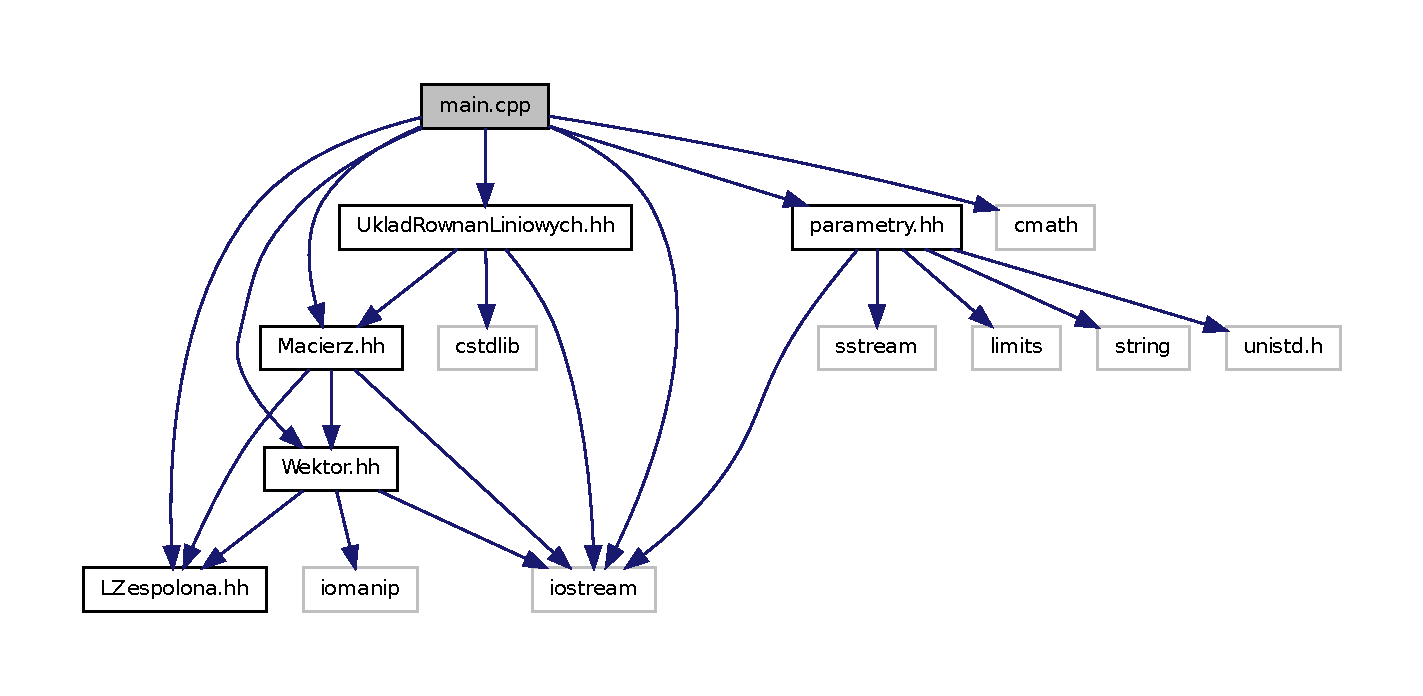
\includegraphics[width=400pt]{main_8cpp__incl}
\end{center}
\end{figure}
\subsection*{Funkcje}
\begin{DoxyCompactItemize}
\item 
int \hyperlink{main_8cpp_a0ddf1224851353fc92bfbff6f499fa97}{main} (int argc, char $\ast$argv\mbox{[}$\,$\mbox{]})
\end{DoxyCompactItemize}


\subsection{Dokumentacja funkcji}
\hypertarget{main_8cpp_a0ddf1224851353fc92bfbff6f499fa97}{
\index{main.cpp@{main.cpp}!main@{main}}
\index{main@{main}!main.cpp@{main.cpp}}
\subsubsection[{main}]{\setlength{\rightskip}{0pt plus 5cm}int main (
\begin{DoxyParamCaption}
\item[{int}]{ argc, }
\item[{char $\ast$}]{ argv\mbox{[}$\,$\mbox{]}}
\end{DoxyParamCaption}
)}}
\label{main_8cpp_a0ddf1224851353fc92bfbff6f499fa97}


Definicja w linii 10 pliku main.cpp.



Oto graf wywołań dla tej funkcji:\nopagebreak
\begin{figure}[H]
\begin{center}
\leavevmode
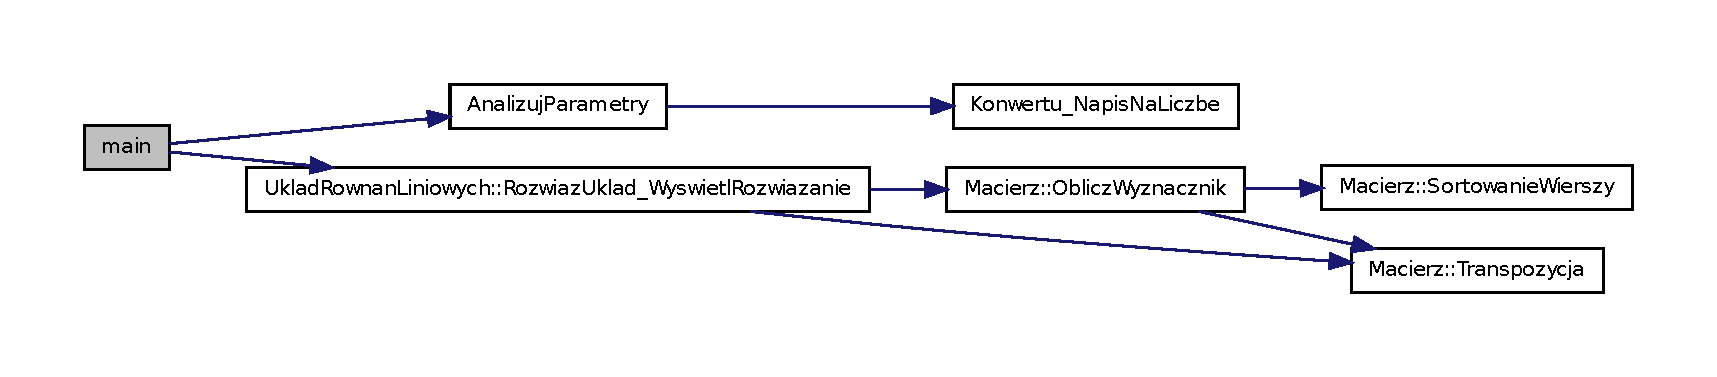
\includegraphics[width=400pt]{main_8cpp_a0ddf1224851353fc92bfbff6f499fa97_cgraph}
\end{center}
\end{figure}



\hypertarget{parametry_8cpp}{
\section{Dokumentacja pliku parametry.cpp}
\label{parametry_8cpp}\index{parametry.cpp@{parametry.cpp}}
}


funkcje sluzacy do przetwarzania argumentow podanych w konsoli  


{\ttfamily \#include \char`\"{}parametry.hh\char`\"{}}\par
Wykres zależności załączania dla parametry.cpp:\nopagebreak
\begin{figure}[H]
\begin{center}
\leavevmode
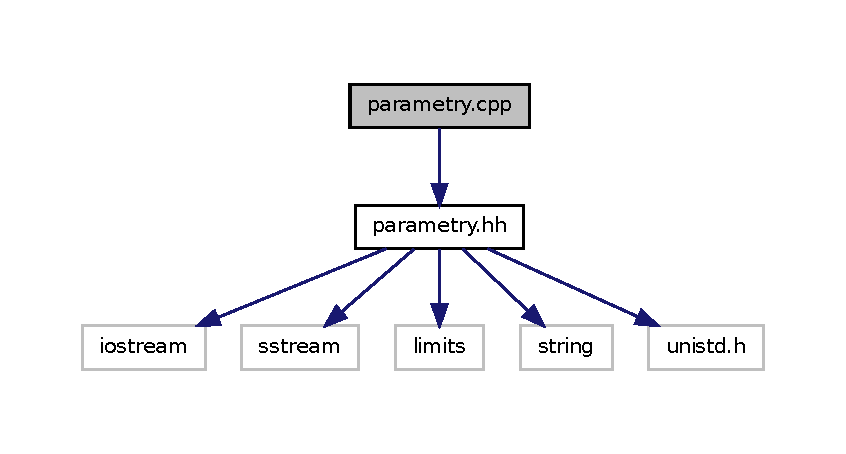
\includegraphics[width=400pt]{parametry_8cpp__incl}
\end{center}
\end{figure}
\subsection*{Definicje}
\begin{DoxyCompactItemize}
\item 
\#define \hyperlink{parametry_8cpp_ac4f92db10fea9b5bd0337dcfa87f1850}{ROZMIAR\_\-LINII}~100
\end{DoxyCompactItemize}
\subsection*{Funkcje}
\begin{DoxyCompactItemize}
\item 
bool \hyperlink{parametry_8cpp_a6a3243d05d7fffdaeba9fefd7549285a}{Konwertu\_\-NapisNaLiczbe} (const char $\ast$wNapis, double \&Liczba)
\begin{DoxyCompactList}\small\item\em Kowertuje napis zawierający znaki cyfr na liczbe reprezentowana przez ten napis. \item\end{DoxyCompactList}\item 
bool \hyperlink{parametry_8cpp_aedf4a4e7e6152bd7ad1c411cf10cef3d}{AnalizujParametry} (int argc, char $\ast$argv\mbox{[}$\,$\mbox{]}, \hyperlink{struct_parametry_wywolania}{ParametryWywolania} \&Param)
\begin{DoxyCompactList}\small\item\em Analizuje parametry linii wywolania i inicjalizuje odpowienie pola w strukturze \char`\"{}ParametryWywolania\char`\"{}, ktore odpowiadaja poszczegolnym parametrom. \item\end{DoxyCompactList}\end{DoxyCompactItemize}


\subsection{Opis szczegółowy}


Definicja w pliku \hyperlink{parametry_8cpp_source}{parametry.cpp}.



\subsection{Dokumentacja definicji}
\hypertarget{parametry_8cpp_ac4f92db10fea9b5bd0337dcfa87f1850}{
\index{parametry.cpp@{parametry.cpp}!ROZMIAR\_\-LINII@{ROZMIAR\_\-LINII}}
\index{ROZMIAR\_\-LINII@{ROZMIAR\_\-LINII}!parametry.cpp@{parametry.cpp}}
\subsubsection[{ROZMIAR\_\-LINII}]{\setlength{\rightskip}{0pt plus 5cm}\#define ROZMIAR\_\-LINII~100}}
\label{parametry_8cpp_ac4f92db10fea9b5bd0337dcfa87f1850}


Definicja w linii 3 pliku parametry.cpp.



\subsection{Dokumentacja funkcji}
\hypertarget{parametry_8cpp_aedf4a4e7e6152bd7ad1c411cf10cef3d}{
\index{parametry.cpp@{parametry.cpp}!AnalizujParametry@{AnalizujParametry}}
\index{AnalizujParametry@{AnalizujParametry}!parametry.cpp@{parametry.cpp}}
\subsubsection[{AnalizujParametry}]{\setlength{\rightskip}{0pt plus 5cm}bool AnalizujParametry (
\begin{DoxyParamCaption}
\item[{int}]{ argc, }
\item[{char $\ast$}]{ argv\mbox{[}$\,$\mbox{]}, }
\item[{{\bf ParametryWywolania} \&}]{ Param}
\end{DoxyParamCaption}
)}}
\label{parametry_8cpp_aedf4a4e7e6152bd7ad1c411cf10cef3d}

\begin{DoxyParams}{Parametry}
\item[\mbox{\tt[in]} {\em argc}]-\/ ilosc parametrow z linii wyolania programu. \item[\mbox{\tt[in]} {\em argv}]-\/ tablica napisow zawieraja (w postaci napisow) poszczegolne parametry wywolania programu. \item[\mbox{\tt[in]} {\em Param}]-\/ jego pola odpowiadaja poszczegolnym parametrom wywolania.\end{DoxyParams}
\begin{DoxyPrecond}{Warunek wstępny}
argc, argv -\/ zawieraja poprawna ilosc i tablice parametrow wywolania.
\end{DoxyPrecond}
\begin{DoxyPostcond}{Warunek końcowy}
Param -\/ zostaje zainicjalizowana zgodnie z lista parametrow wywolania programu (o ile one wystapily). 
\end{DoxyPostcond}
\begin{DoxyReturn}{Zwraca}
true -\/ jeśli operacja się powiodła, tzn. wszystkie opcje wywołania i ich parametry są poprawne, 

false -\/ w przypadku przeciwnym. 
\end{DoxyReturn}


Definicja w linii 55 pliku parametry.cpp.



Oto graf wywołań dla tej funkcji:\nopagebreak
\begin{figure}[H]
\begin{center}
\leavevmode
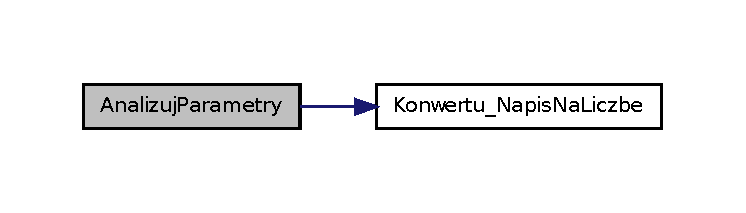
\includegraphics[width=358pt]{parametry_8cpp_aedf4a4e7e6152bd7ad1c411cf10cef3d_cgraph}
\end{center}
\end{figure}


\hypertarget{parametry_8cpp_a6a3243d05d7fffdaeba9fefd7549285a}{
\index{parametry.cpp@{parametry.cpp}!Konwertu\_\-NapisNaLiczbe@{Konwertu\_\-NapisNaLiczbe}}
\index{Konwertu\_\-NapisNaLiczbe@{Konwertu\_\-NapisNaLiczbe}!parametry.cpp@{parametry.cpp}}
\subsubsection[{Konwertu\_\-NapisNaLiczbe}]{\setlength{\rightskip}{0pt plus 5cm}bool Konwertu\_\-NapisNaLiczbe (
\begin{DoxyParamCaption}
\item[{const char $\ast$}]{ wNapis, }
\item[{double \&}]{ Liczba}
\end{DoxyParamCaption}
)}}
\label{parametry_8cpp_a6a3243d05d7fffdaeba9fefd7549285a}

\begin{DoxyParams}{Parametry}
\item[\mbox{\tt[in]} {\em wNapis}]-\/ wskaznik na napis reprezentujacy liczbe calkowita, \item[\mbox{\tt[in]} {\em Liczba}]-\/ wpiswany jest do tego parametru wynik konwersji napisu na liczbe.\end{DoxyParams}
\begin{DoxyPrecond}{Warunek wstępny}
Napis musi zawierac ciag cyfr, ktore nie sa oddzielne spacjami. 

Musi on reprezntowac liczbe calkowita, ktora miesci sie w przedziale wartosci typu int.
\end{DoxyPrecond}
\begin{DoxyReturn}{Zwraca}
true -\/ jesli operacja konwersji zakonczyla sie poprawnie, 

false -\/ w przypadku przeciwnym. 
\end{DoxyReturn}


Definicja w linii 25 pliku parametry.cpp.


\hypertarget{parametry_8hh}{
\section{Dokumentacja pliku parametry.hh}
\label{parametry_8hh}\index{parametry.hh@{parametry.hh}}
}


Struktura zawiera wszystkie pola odpowiadajace parametrom z jakimi moze zostac wywolany program. Posiada funkcje analizujaca parametry i Konwertujaca napis na liczbe.  


{\ttfamily \#include $<$iostream$>$}\par
{\ttfamily \#include $<$sstream$>$}\par
{\ttfamily \#include $<$limits$>$}\par
{\ttfamily \#include $<$string$>$}\par
{\ttfamily \#include $<$unistd.h$>$}\par
Wykres zależności załączania dla parametry.hh:\nopagebreak
\begin{figure}[H]
\begin{center}
\leavevmode
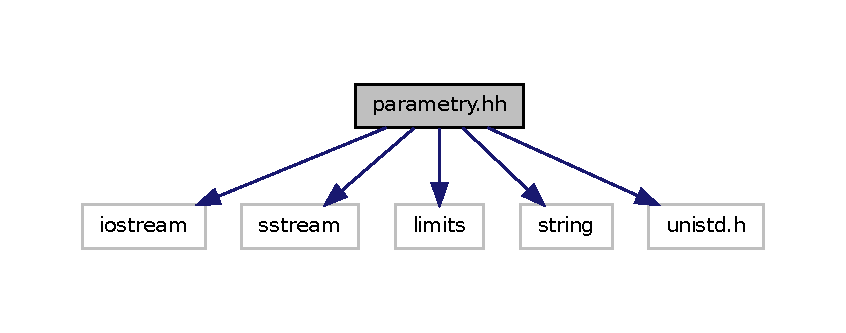
\includegraphics[width=400pt]{parametry_8hh__incl}
\end{center}
\end{figure}
Ten wykres pokazuje, które pliki bezpośrednio lub pośrednio załączają ten plik:\nopagebreak
\begin{figure}[H]
\begin{center}
\leavevmode
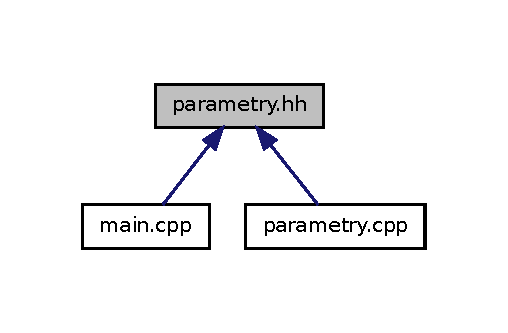
\includegraphics[width=244pt]{parametry_8hh__dep__incl}
\end{center}
\end{figure}
\subsection*{Komponenty}
\begin{DoxyCompactItemize}
\item 
struct \hyperlink{struct_parametry_wywolania}{ParametryWywolania}
\end{DoxyCompactItemize}
\subsection*{Definicje}
\begin{DoxyCompactItemize}
\item 
\#define \hyperlink{parametry_8hh_ac4f92db10fea9b5bd0337dcfa87f1850}{ROZMIAR\_\-LINII}~100
\end{DoxyCompactItemize}
\subsection*{Funkcje}
\begin{DoxyCompactItemize}
\item 
bool \hyperlink{parametry_8hh_a6a3243d05d7fffdaeba9fefd7549285a}{Konwertu\_\-NapisNaLiczbe} (const char $\ast$wNapis, double \&Liczba)
\begin{DoxyCompactList}\small\item\em Kowertuje napis zawierający znaki cyfr na liczbe reprezentowana przez ten napis. \item\end{DoxyCompactList}\item 
bool \hyperlink{parametry_8hh_aedf4a4e7e6152bd7ad1c411cf10cef3d}{AnalizujParametry} (int argc, char $\ast$argv\mbox{[}$\,$\mbox{]}, \hyperlink{struct_parametry_wywolania}{ParametryWywolania} \&Param)
\begin{DoxyCompactList}\small\item\em Analizuje parametry linii wywolania i inicjalizuje odpowienie pola w strukturze \char`\"{}ParametryWywolania\char`\"{}, ktore odpowiadaja poszczegolnym parametrom. \item\end{DoxyCompactList}\end{DoxyCompactItemize}


\subsection{Opis szczegółowy}


Definicja w pliku \hyperlink{parametry_8hh_source}{parametry.hh}.



\subsection{Dokumentacja definicji}
\hypertarget{parametry_8hh_ac4f92db10fea9b5bd0337dcfa87f1850}{
\index{parametry.hh@{parametry.hh}!ROZMIAR\_\-LINII@{ROZMIAR\_\-LINII}}
\index{ROZMIAR\_\-LINII@{ROZMIAR\_\-LINII}!parametry.hh@{parametry.hh}}
\subsubsection[{ROZMIAR\_\-LINII}]{\setlength{\rightskip}{0pt plus 5cm}\#define ROZMIAR\_\-LINII~100}}
\label{parametry_8hh_ac4f92db10fea9b5bd0337dcfa87f1850}


Definicja w linii 10 pliku parametry.hh.



\subsection{Dokumentacja funkcji}
\hypertarget{parametry_8hh_aedf4a4e7e6152bd7ad1c411cf10cef3d}{
\index{parametry.hh@{parametry.hh}!AnalizujParametry@{AnalizujParametry}}
\index{AnalizujParametry@{AnalizujParametry}!parametry.hh@{parametry.hh}}
\subsubsection[{AnalizujParametry}]{\setlength{\rightskip}{0pt plus 5cm}bool AnalizujParametry (
\begin{DoxyParamCaption}
\item[{int}]{ argc, }
\item[{char $\ast$}]{ argv\mbox{[}$\,$\mbox{]}, }
\item[{{\bf ParametryWywolania} \&}]{ Param}
\end{DoxyParamCaption}
)}}
\label{parametry_8hh_aedf4a4e7e6152bd7ad1c411cf10cef3d}

\begin{DoxyParams}{Parametry}
\item[\mbox{\tt[in]} {\em argc}]-\/ ilosc parametrow z linii wyolania programu. \item[\mbox{\tt[in]} {\em argv}]-\/ tablica napisow zawieraja (w postaci napisow) poszczegolne parametry wywolania programu. \item[\mbox{\tt[in]} {\em Param}]-\/ jego pola odpowiadaja poszczegolnym parametrom wywolania.\end{DoxyParams}
\begin{DoxyPrecond}{Warunek wstępny}
argc, argv -\/ zawieraja poprawna ilosc i tablice parametrow wywolania.
\end{DoxyPrecond}
\begin{DoxyPostcond}{Warunek końcowy}
Param -\/ zostaje zainicjalizowana zgodnie z lista parametrow wywolania programu (o ile one wystapily). 
\end{DoxyPostcond}
\begin{DoxyReturn}{Zwraca}
true -\/ jeśli operacja się powiodła, tzn. wszystkie opcje wywołania i ich parametry są poprawne, 

false -\/ w przypadku przeciwnym. 
\end{DoxyReturn}


Definicja w linii 55 pliku parametry.cpp.



Oto graf wywołań dla tej funkcji:\nopagebreak
\begin{figure}[H]
\begin{center}
\leavevmode
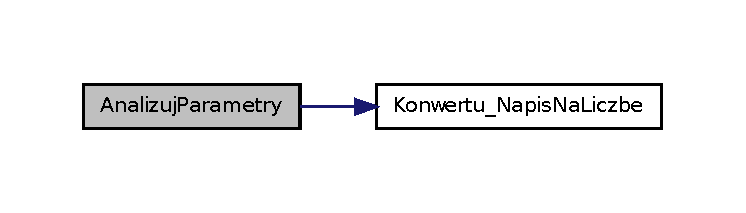
\includegraphics[width=358pt]{parametry_8hh_aedf4a4e7e6152bd7ad1c411cf10cef3d_cgraph}
\end{center}
\end{figure}


\hypertarget{parametry_8hh_a6a3243d05d7fffdaeba9fefd7549285a}{
\index{parametry.hh@{parametry.hh}!Konwertu\_\-NapisNaLiczbe@{Konwertu\_\-NapisNaLiczbe}}
\index{Konwertu\_\-NapisNaLiczbe@{Konwertu\_\-NapisNaLiczbe}!parametry.hh@{parametry.hh}}
\subsubsection[{Konwertu\_\-NapisNaLiczbe}]{\setlength{\rightskip}{0pt plus 5cm}bool Konwertu\_\-NapisNaLiczbe (
\begin{DoxyParamCaption}
\item[{const char $\ast$}]{ wNapis, }
\item[{double \&}]{ Liczba}
\end{DoxyParamCaption}
)}}
\label{parametry_8hh_a6a3243d05d7fffdaeba9fefd7549285a}

\begin{DoxyParams}{Parametry}
\item[\mbox{\tt[in]} {\em wNapis}]-\/ wskaznik na napis reprezentujacy liczbe calkowita, \item[\mbox{\tt[in]} {\em Liczba}]-\/ wpiswany jest do tego parametru wynik konwersji napisu na liczbe.\end{DoxyParams}
\begin{DoxyPrecond}{Warunek wstępny}
Napis musi zawierac ciag cyfr, ktore nie sa oddzielne spacjami. 

Musi on reprezntowac liczbe calkowita, ktora miesci sie w przedziale wartosci typu int.
\end{DoxyPrecond}
\begin{DoxyReturn}{Zwraca}
true -\/ jesli operacja konwersji zakonczyla sie poprawnie, 

false -\/ w przypadku przeciwnym. 
\end{DoxyReturn}


Definicja w linii 25 pliku parametry.cpp.


\hypertarget{strona-01-diagram-klas_8dox}{
\section{Dokumentacja pliku strona-\/01-\/diagram-\/klas.dox}
\label{strona-01-diagram-klas_8dox}\index{strona-\/01-\/diagram-\/klas.dox@{strona-\/01-\/diagram-\/klas.dox}}
}

\hypertarget{strona-glowna_8dox}{
\section{Dokumentacja pliku strona-\/glowna.dox}
\label{strona-glowna_8dox}\index{strona-\/glowna.dox@{strona-\/glowna.dox}}
}

\hypertarget{_uklad_rownan_liniowych_8hh}{
\section{Dokumentacja pliku UkladRownanLiniowych.hh}
\label{_uklad_rownan_liniowych_8hh}\index{UkladRownanLiniowych.hh@{UkladRownanLiniowych.hh}}
}


Klasa \hyperlink{class_uklad_rownan_liniowych}{UkladRownanLiniowych} modeluje w programie \hyperlink{class_macierz}{Macierz} wspolczynnikow rownania, wektor wyrazow wolnych. Sklada sie z metody do rozwiazania ukladu i wyswietlenia tego rozwiazania.  


{\ttfamily \#include \char`\"{}Macierz.hh\char`\"{}}\par
{\ttfamily \#include $<$iostream$>$}\par
{\ttfamily \#include $<$cstdlib$>$}\par
Wykres zależności załączania dla UkladRownanLiniowych.hh:\nopagebreak
\begin{figure}[H]
\begin{center}
\leavevmode
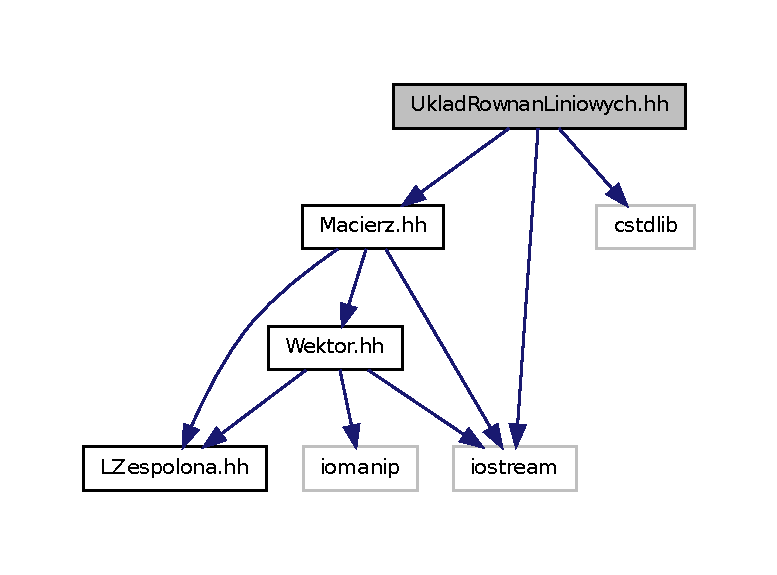
\includegraphics[width=373pt]{_uklad_rownan_liniowych_8hh__incl}
\end{center}
\end{figure}
Ten wykres pokazuje, które pliki bezpośrednio lub pośrednio załączają ten plik:\nopagebreak
\begin{figure}[H]
\begin{center}
\leavevmode
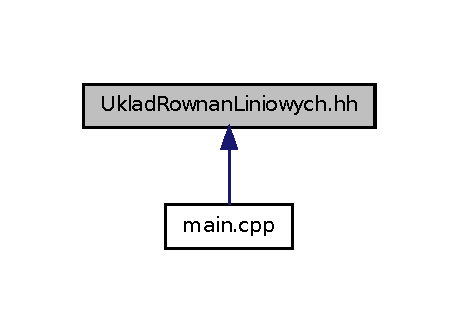
\includegraphics[width=220pt]{_uklad_rownan_liniowych_8hh__dep__incl}
\end{center}
\end{figure}
\subsection*{Komponenty}
\begin{DoxyCompactItemize}
\item 
class \hyperlink{class_uklad_rownan_liniowych}{UkladRownanLiniowych$<$ Typ, ROZMIAR $>$}
\end{DoxyCompactItemize}
\subsection*{Funkcje}
\begin{DoxyCompactItemize}
\item 
{\footnotesize template$<$typename Typ , int ROZMIAR$>$ }\\istream \& \hyperlink{_uklad_rownan_liniowych_8hh_a8466044dc69ceaec3b324caeeb95cb2d}{operator$>$$>$} (istream \&Strm, \hyperlink{class_uklad_rownan_liniowych}{UkladRownanLiniowych}$<$ Typ, ROZMIAR $>$ \&UklRown)
\begin{DoxyCompactList}\small\item\em Szablon funkcji operatorowej $>$$>$ sluzy do wczytywania calego wyrazenia (tj macierzy wspolczynnikow oraz wektora wyrazow wolnych podanych przez uzytkownika). \item\end{DoxyCompactList}\item 
{\footnotesize template$<$typename Typ , int ROZMIAR$>$ }\\ostream \& \hyperlink{_uklad_rownan_liniowych_8hh_aeedb2b3cdaffd4a69b18541d24d94dd1}{operator$<$$<$} (ostream \&Strm, const \hyperlink{class_uklad_rownan_liniowych}{UkladRownanLiniowych}$<$ Typ, ROZMIAR $>$ \&UklRown)
\begin{DoxyCompactList}\small\item\em Szablon funkcji operatorowej $<$$<$ sluzy do wypisywania na strumien wyjsciowy calego wyrazenia skladajacego sie z liczb znajdujacych sie w pamieci. \item\end{DoxyCompactList}\end{DoxyCompactItemize}


\subsection{Opis szczegółowy}


Definicja w pliku \hyperlink{_uklad_rownan_liniowych_8hh_source}{UkladRownanLiniowych.hh}.



\subsection{Dokumentacja funkcji}
\hypertarget{_uklad_rownan_liniowych_8hh_aeedb2b3cdaffd4a69b18541d24d94dd1}{
\index{UkladRownanLiniowych.hh@{UkladRownanLiniowych.hh}!operator$<$$<$@{operator$<$$<$}}
\index{operator$<$$<$@{operator$<$$<$}!UkladRownanLiniowych.hh@{UkladRownanLiniowych.hh}}
\subsubsection[{operator$<$$<$}]{\setlength{\rightskip}{0pt plus 5cm}template$<$typename Typ , int ROZMIAR$>$ ostream\& operator$<$$<$ (
\begin{DoxyParamCaption}
\item[{ostream \&}]{ Strm, }
\item[{const {\bf UkladRownanLiniowych}$<$ Typ, ROZMIAR $>$ \&}]{ UklRown}
\end{DoxyParamCaption}
)}}
\label{_uklad_rownan_liniowych_8hh_aeedb2b3cdaffd4a69b18541d24d94dd1}
\begin{DoxyReturn}{Zwraca}
referencja do strumienia wyjsciowego 
\end{DoxyReturn}

\begin{DoxyParams}{Parametry}
\item[\mbox{\tt[in,out]} {\em \&Strm}]-\/ referencja do strumienia wyjsciowego \item[\mbox{\tt[in,out]} {\em \&UklRown}]-\/ referencja do szablonu klasy typu \hyperlink{class_uklad_rownan_liniowych}{UkladRownanLiniowych} \end{DoxyParams}
\begin{DoxyPrecond}{Warunek wstępny}
Wymagane uprzednie wczytanie liczb w ilosci 
\end{DoxyPrecond}


Definicja w linii 69 pliku UkladRownanLiniowych.hh.

\hypertarget{_uklad_rownan_liniowych_8hh_a8466044dc69ceaec3b324caeeb95cb2d}{
\index{UkladRownanLiniowych.hh@{UkladRownanLiniowych.hh}!operator$>$$>$@{operator$>$$>$}}
\index{operator$>$$>$@{operator$>$$>$}!UkladRownanLiniowych.hh@{UkladRownanLiniowych.hh}}
\subsubsection[{operator$>$$>$}]{\setlength{\rightskip}{0pt plus 5cm}template$<$typename Typ , int ROZMIAR$>$ istream\& operator$>$$>$ (
\begin{DoxyParamCaption}
\item[{istream \&}]{ Strm, }
\item[{{\bf UkladRownanLiniowych}$<$ Typ, ROZMIAR $>$ \&}]{ UklRown}
\end{DoxyParamCaption}
)}}
\label{_uklad_rownan_liniowych_8hh_a8466044dc69ceaec3b324caeeb95cb2d}
\begin{DoxyReturn}{Zwraca}
referencja do strumienia wejsciowego 
\end{DoxyReturn}

\begin{DoxyParams}{Parametry}
\item[\mbox{\tt[in,out]} {\em \&Strm}]-\/ referencja do strumienia wejsciowego \item[\mbox{\tt[in,out]} {\em \&UklRown}]-\/ referencja do szablonu klasy typu \hyperlink{class_uklad_rownan_liniowych}{UkladRownanLiniowych} \end{DoxyParams}


Definicja w linii 54 pliku UkladRownanLiniowych.hh.


\hypertarget{_wektor_8hh}{
\section{Dokumentacja pliku Wektor.hh}
\label{_wektor_8hh}\index{Wektor.hh@{Wektor.hh}}
}


Szablon Klasy wektor modeluje wektor w programie, przechowuje go jako 3elementowa tablice typu double Jej metody to operacje arytmetyczne na wektorach.  


{\ttfamily \#include $<$iomanip$>$}\par
{\ttfamily \#include $<$iostream$>$}\par
{\ttfamily \#include \char`\"{}LZespolona.hh\char`\"{}}\par
Wykres zależności załączania dla Wektor.hh:\nopagebreak
\begin{figure}[H]
\begin{center}
\leavevmode
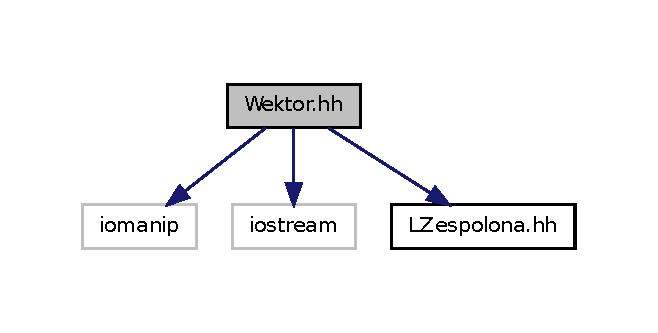
\includegraphics[width=316pt]{_wektor_8hh__incl}
\end{center}
\end{figure}
Ten wykres pokazuje, które pliki bezpośrednio lub pośrednio załączają ten plik:\nopagebreak
\begin{figure}[H]
\begin{center}
\leavevmode
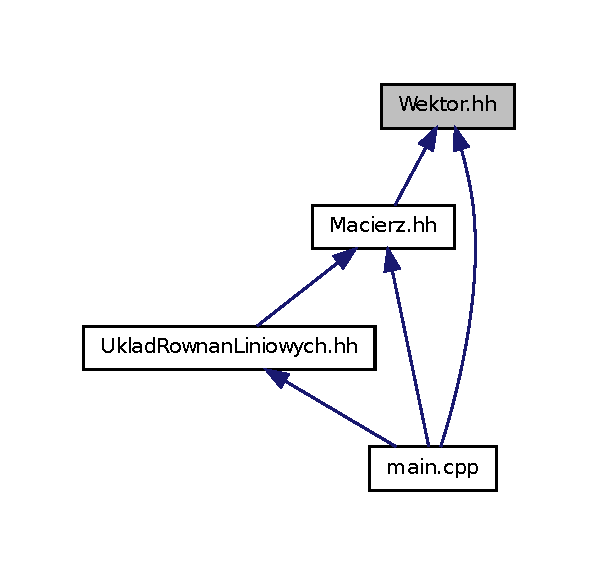
\includegraphics[width=287pt]{_wektor_8hh__dep__incl}
\end{center}
\end{figure}
\subsection*{Komponenty}
\begin{DoxyCompactItemize}
\item 
class \hyperlink{class_wektor}{Wektor$<$ Typ, ROZMIAR $>$}
\end{DoxyCompactItemize}
\subsection*{Funkcje}
\begin{DoxyCompactItemize}
\item 
{\footnotesize template$<$typename Typ , int ROZMIAR$>$ }\\std::istream \& \hyperlink{_wektor_8hh_a819aa25942acc1bc4adcbc6e63081d39}{operator$>$$>$} (std::istream \&Strm, \hyperlink{class_wektor}{Wektor}$<$ Typ, ROZMIAR $>$ \&Wek)
\begin{DoxyCompactList}\small\item\em Szablon funkcji operatorowej $>$$>$ sluzy do wczytywania wektora skladajacego sie z liczb podanych przez uzytkownika. \item\end{DoxyCompactList}\item 
{\footnotesize template$<$typename Typ , int ROZMIAR$>$ }\\std::ostream \& \hyperlink{_wektor_8hh_ad9cda9bedc161ef0997004ec02402850}{operator$<$$<$} (std::ostream \&Strm, const \hyperlink{class_wektor}{Wektor}$<$ Typ, ROZMIAR $>$ \&Wek)
\begin{DoxyCompactList}\small\item\em Szablon funkcji operatorowej $<$$<$ sluzy do wypisywanie na strumien wejsciowy wektora sladajacego sie z liczb znajdujacych sie w pamieci. \item\end{DoxyCompactList}\item 
{\footnotesize template$<$typename Typ , int ROZMIAR$>$ }\\\hyperlink{class_wektor}{Wektor}$<$ Typ, ROZMIAR $>$ \hyperlink{_wektor_8hh_a7c5d0bef7270148f7dcc5629c0728deb}{operator$\ast$} (const double Liczba, const \hyperlink{class_wektor}{Wektor}$<$ Typ, ROZMIAR $>$ \_\-V)
\begin{DoxyCompactList}\small\item\em Szablon funkcji operatorowej $\ast$ sluzy do mnozenia liczby przez wektor. \item\end{DoxyCompactList}\end{DoxyCompactItemize}


\subsection{Opis szczegółowy}


Definicja w pliku \hyperlink{_wektor_8hh_source}{Wektor.hh}.



\subsection{Dokumentacja funkcji}
\hypertarget{_wektor_8hh_a7c5d0bef7270148f7dcc5629c0728deb}{
\index{Wektor.hh@{Wektor.hh}!operator$\ast$@{operator$\ast$}}
\index{operator$\ast$@{operator$\ast$}!Wektor.hh@{Wektor.hh}}
\subsubsection[{operator$\ast$}]{\setlength{\rightskip}{0pt plus 5cm}template$<$typename Typ , int ROZMIAR$>$ {\bf Wektor}$<$Typ,ROZMIAR$>$ operator$\ast$ (
\begin{DoxyParamCaption}
\item[{const double}]{ Liczba, }
\item[{const {\bf Wektor}$<$ Typ, ROZMIAR $>$}]{ \_\-V}
\end{DoxyParamCaption}
)}}
\label{_wektor_8hh_a7c5d0bef7270148f7dcc5629c0728deb}
\begin{DoxyReturn}{Zwraca}
referencja \hyperlink{class_wektor}{Wektor} 
\end{DoxyReturn}

\begin{DoxyParams}{Parametry}
\item[\mbox{\tt[in]} {\em Liczba}]-\/ liczba rzeczywista \item[\mbox{\tt[in]} {\em \_\-V}]-\/ wektor \end{DoxyParams}
\begin{DoxyPrecond}{Warunek wstępny}
poprawne wczytanie wektora i podanie liczby 
\end{DoxyPrecond}
\begin{DoxyReturn}{Zwraca}
mnozenie liczby przez wektor, wynik jako wartosc zwracana przez funkcje 
\end{DoxyReturn}


Definicja w linii 121 pliku Wektor.hh.

\hypertarget{_wektor_8hh_ad9cda9bedc161ef0997004ec02402850}{
\index{Wektor.hh@{Wektor.hh}!operator$<$$<$@{operator$<$$<$}}
\index{operator$<$$<$@{operator$<$$<$}!Wektor.hh@{Wektor.hh}}
\subsubsection[{operator$<$$<$}]{\setlength{\rightskip}{0pt plus 5cm}template$<$typename Typ , int ROZMIAR$>$ std::ostream\& operator$<$$<$ (
\begin{DoxyParamCaption}
\item[{std::ostream \&}]{ Strm, }
\item[{const {\bf Wektor}$<$ Typ, ROZMIAR $>$ \&}]{ Wek}
\end{DoxyParamCaption}
)}}
\label{_wektor_8hh_ad9cda9bedc161ef0997004ec02402850}
\begin{DoxyReturn}{Zwraca}
referencja do strumienia wejsciowego 
\end{DoxyReturn}

\begin{DoxyParams}{Parametry}
\item[\mbox{\tt[in,out]} {\em \&Strm}]-\/ referencja do strumienia wejsciowego \item[\mbox{\tt[in,out]} {\em \&Wek}]-\/ referencja do szablonu klasy typu \hyperlink{class_wektor}{Wektor} \end{DoxyParams}


Definicja w linii 89 pliku Wektor.hh.

\hypertarget{_wektor_8hh_a819aa25942acc1bc4adcbc6e63081d39}{
\index{Wektor.hh@{Wektor.hh}!operator$>$$>$@{operator$>$$>$}}
\index{operator$>$$>$@{operator$>$$>$}!Wektor.hh@{Wektor.hh}}
\subsubsection[{operator$>$$>$}]{\setlength{\rightskip}{0pt plus 5cm}template$<$typename Typ , int ROZMIAR$>$ std::istream\& operator$>$$>$ (
\begin{DoxyParamCaption}
\item[{std::istream \&}]{ Strm, }
\item[{{\bf Wektor}$<$ Typ, ROZMIAR $>$ \&}]{ Wek}
\end{DoxyParamCaption}
)}}
\label{_wektor_8hh_a819aa25942acc1bc4adcbc6e63081d39}
\begin{DoxyReturn}{Zwraca}
referancja do strumienia wejsciowego 
\end{DoxyReturn}

\begin{DoxyParams}{Parametry}
\item[\mbox{\tt[in,out]} {\em \&Strm}]-\/ referencja do strumienia wejsciowego \item[\mbox{\tt[in,out]} {\em \&Wek}]-\/ referencja do szablonu klasy typu \hyperlink{class_wektor}{Wektor} \end{DoxyParams}
\begin{DoxyPrecond}{Warunek wstępny}
Wymagane sa liczby w ilosci stalej ROZMIAR 
\end{DoxyPrecond}


Definicja w linii 75 pliku Wektor.hh.


\printindex
\end{document}
